% Plantilla para un Trabajo Fin de Grado de la Universidad de Granada,
% ingeniería informática.
%
%  Autor: Andrés Arco
%  Licencia: GNU GPLv2.
%
% Esta plantilla es una adaptación al castellano de la plantilla
% classicthesis de André Miede, que puede obtenerse en:
%  https://ctan.org/tex-archive/macros/latex/contrib/classicthesis?lang=en
% La plantilla original se licencia en GNU GPLv2.
%
% Esta plantilla usa símbolos de la Universidad de Granada sujetos a la normativa
% de identidad visual corporativa, que puede encontrarse en:
% http://secretariageneral.ugr.es/pages/ivc/normativa
%
% La compilación se realiza con las siguientes instrucciones:
%   pdflatex --shell-escape main.tex
%   bibtex main
%   pdflatex --shell-escape main.tex

% Opciones del tipo de documento
\documentclass[oneside,openright,titlepage,numbers=noenddot,openany,headinclude,footinclude=true,
cleardoublepage=empty,abstractoff,BCOR=5mm,paper=a4,fontsize=12pt,main=spanish]{scrreprt}

% Paquetes de latex que se cargan al inicio. Cubren la entrada de
% texto, gráficos, código fuente y símbolos.
\usepackage[utf8]{inputenc}
\usepackage[T1]{fontenc}
\usepackage{multirow}
\usepackage{upgreek}
\usepackage{graphicx} % Inclusión de imágenes.
\usepackage{grffile}  % Distintos formatos para imágenes.
\usepackage{longtable} % Tablas multipágina.
\usepackage{wrapfig} % Coloca texto alrededor de una figura.
\usepackage{rotating}
\usepackage[normalem]{ulem}
\usepackage{amsmath}
\usepackage{textcomp}
\usepackage{amssymb}
\usepackage{capt-of}
\usepackage[colorlinks=true]{hyperref}
\usepackage{tikz} % Diagramas conmutativos.
\usetikzlibrary{cd,shapes.geometric}
\usepackage{minted} % Código fuente.
\usepackage[T1]{fontenc}
\usepackage{natbib}
\usepackage[toc,page]{appendix}

\tikzcdset{m/.style={column sep=0pt,
    every arrow/.style={draw,thick,-latex,minimum height=1.0em},
    /tikz/w/.style={fill=white},
    cells={nodes={circle,inner sep=-0.5pt,fill=gray!30,draw,minimum height=2em}}}}  

% Plantilla classicthesis
\usepackage[beramono,eulerchapternumbers,linedheaders,parts,a5paper,dottedtoc,
manychapters,pdfspacing]{classicthesis}

% Geometría y espaciado de párrafos.
\setcounter{secnumdepth}{0}
\usepackage{enumitem}
\setitemize{noitemsep,topsep=0pt,parsep=0pt,partopsep=0pt}
\setlist[enumerate]{topsep=0pt,itemsep=-1ex,partopsep=1ex,parsep=1ex}
\usepackage[top=1in, bottom=1.5in, left=1in, right=1in]{geometry}
\setlength\itemsep{0em}
\setlength{\parindent}{0pt}
\usepackage{parskip}

% Profundidad de la tabla de contenidos.
\setcounter{secnumdepth}{3}

% Usa el paquete minted para mostrar trozos de código.
% Pueden seleccionarse el lenguaje apropiado y el estilo del código.
\usepackage{minted}
\usemintedstyle{colorful}
\setminted{fontsize=\small}
\setminted[python]{linenos=false,fontsize=\small}
\renewcommand{\theFancyVerbLine}{\sffamily\textcolor[rgb]{0.5,0.5,1.0}{\oldstylenums{\arabic{FancyVerbLine}}}}

% Archivos de configuración.
%------------------------
% Bibliotecas para matemáticas de latex
%------------------------
\usepackage{amsthm}
\usepackage{amsmath}
\usepackage[ruled, spanish, onelanguage]{algorithm2e}
\usepackage{tikz}
\usepackage{tikz-cd}
\usetikzlibrary{shapes, fit, automata,  positioning, arrows}
\usepackage{bussproofs}
\EnableBpAbbreviations{}
\usepackage{mathtools}
\usepackage{scalerel}
\usepackage{verbatim} % comentarios
\usepackage{stmaryrd}
\usepackage{natbib}
\usepackage{bm}
\usepackage{hyperref}
\usepackage{amsthm}
\usepackage[theorems, skins, breakable]{tcolorbox}

% Licencia
\usepackage[
    type={CC},
    modifier={by-sa},
    version={4.0},
]{doclicense}

% Glossaries
%\usepackage[toc, nopostdot,  style=super, nonumberlist, section=chapter ]{glossaries}
%\newglossary{symbols}{sym}{sbl}{List of Abbreviations and Symbols}
%\makeglossaries
%\loadglsentries{bibliography/glossary}

%------------------------
% Estilos para los teoremas
%------------------------
\theoremstyle{definition}
\newtheorem{theorem}{Teorema}
\newtheorem{proposition}{Proposición}
\newtheorem{lemma}{Lema}
\newtheorem{corollary}{Corolario}
\newtheorem{definition}{Definición}
\theoremstyle{remark}
\newtheorem{remark}{Comentario}
\newtheorem{example}{Ejemplo}
\newtheorem{result}{Resultado}
\theoremstyle{definition}
\newtheorem{notation}{Notación}

\tcolorboxenvironment{definition}{
  blanker,
  breakable,
  left=12pt,
  %before skip=12pt,
  after skip=12pt,
  borderline west={2pt}{0pt},
  before upper={\parindent 12pt}
}

\tcolorboxenvironment{proposition}{
  blanker,
  breakable,
  left=12pt,
  %before skip=12pt,
  after skip=12pt,
  borderline west={2pt}{0pt},
  before upper={\parindent 12pt}
}

\tcolorboxenvironment{theorem}{
  blanker,
  breakable,
  left=12pt,
  %before skip=12pt,
  after skip=12pt,
  borderline west={2pt}{0pt}{red},
  before upper={\parindent 12pt}
}

\tcolorboxenvironment{corollary}{
  blanker,
  breakable,
  left=12pt,
  %before skip=12pt,
  after skip=12pt,
  borderline west={2pt}{0pt}{red},
  before upper={\parindent 12pt}
}

\tcolorboxenvironment{lemma}{
  blanker,
  breakable,
  left=12pt,
  %before skip=12pt,
  after skip=12pt,
  borderline west={2pt}{0pt}{red},
  before upper={\parindent 12pt}
}

\begingroup\makeatletter\@for\theoremstyle:=definition,remark,lemma,plain\do{\expandafter\g@addto@macro\csname th@\theoremstyle\endcsname{\addtolength\thm@preskip\parskip}}\endgroup

%------------------------
% Macros
% ------------------------

% Aquí pueden añadirse abreviaturas para comandos de latex
% frequentemente usados.
\newcommand*\diff{\mathop{}\!\mathrm{d}}
\newcommand\ddfrac[2]{\frac{\displaystyle #1}{\displaystyle #2}}
\newcommand{\abs}[1]{\left\lvert#1\right\rvert} 
\newcommand{\norm}[1]{\left\lVert#1\right\rVert}
\newcommand{\norminf}[1]{\left \| #1 \right \|_\infty} 
\newcommand{\KN}{\mathbb K^{\mathbb N}}
\newcommand{\RN}{\mathbb R^{\mathbb N}}
\newcommand{\K}{\mathbb K}
\newcommand{\N}{\mathbb N}
\newcommand{\R}{\mathbb{R}}
\newcommand{\D}{\ \mathrm d}
\newcommand{\Ro}{\R_0^+}
\newcommand{\M}{\mathcal{M}}
\newcommand{\PR}{\mathcal{P}(\R^N)}
\newcommand{\mst}{(X_1,\dots,X_n)}
\newcommand{\htheta}{\bm{\hat{\theta}}}
\newcommand{\Rn}{\R^N}
\newcommand{\nm}[1]{ \textbf{#1}}
\newcommand{\btheta}{\bm{\theta}}
\newcommand{\bigCI}{\mathrel{\text{\scalebox{1.07}{$\perp\mkern-10mu\perp$}}}}
\newcommand\restr[2]{{% we make the whole thing an ordinary symbol
  \left.\kern-\nulldelimiterspace % automatically resize the bar with \right
  #1 % the function
  \vphantom{\big|} % pretend it's a little taller at normal size
  \right|_{#2} % this is the delimiter
  }}
\newcommand\mm[3][]{\begin{tabular}{@{}c@{}}
  \ensuremath{\textbf{#2}}\\[-1.2ex]{\text{\tiny(#3)}}
  \end{tabular}}
  % En macros.tex se almacenan las opciones y comandos para escribir matemáticas.
\graphicspath{ {./images/} }
% ****************************************************************************************************
% classicthesis-config.tex 
% formerly known as loadpackages.sty, classicthesis-ldpkg.sty, and classicthesis-preamble.sty 
% Use it at the beginning of your ClassicThesis.tex, or as a LaTeX Preamble 
% in your ClassicThesis.{tex,lyx} with % ****************************************************************************************************
% classicthesis-config.tex 
% formerly known as loadpackages.sty, classicthesis-ldpkg.sty, and classicthesis-preamble.sty 
% Use it at the beginning of your ClassicThesis.tex, or as a LaTeX Preamble 
% in your ClassicThesis.{tex,lyx} with % ****************************************************************************************************
% classicthesis-config.tex 
% formerly known as loadpackages.sty, classicthesis-ldpkg.sty, and classicthesis-preamble.sty 
% Use it at the beginning of your ClassicThesis.tex, or as a LaTeX Preamble 
% in your ClassicThesis.{tex,lyx} with \input{classicthesis-config}
% ****************************************************************************************************  
% If you like the classicthesis, then I would appreciate a postcard. 
% My address can be found in the file ClassicThesis.pdf. A collection 
% of the postcards I received so far is available online at 
% http://postcards.miede.de
% ****************************************************************************************************


% ****************************************************************************************************
% 0. Set the encoding of your files. UTF-8 is the only sensible encoding nowadays. If you can't read
% äöüßáéçèê∂åëæƒÏ€ then change the encoding setting in your editor, not the line below. If your editor
% does not support utf8 use another editor!
% ****************************************************************************************************
\PassOptionsToPackage{utf8x}{inputenc}
	\usepackage{inputenc}

% ****************************************************************************************************
% 1. Configure classicthesis for your needs here, e.g., remove "drafting" below 
% in order to deactivate the time-stamp on the pages
% ****************************************************************************************************
\PassOptionsToPackage{eulerchapternumbers,listings,drafting,%
		pdfspacing,%floatperchapter,%linedheaders,%
                subfig,beramono,eulermath,parts,dottedtoc}{classicthesis}   

% ********************************************************************
% Available options for classicthesis.sty 
% (see ClassicThesis.pdf for more information):
% drafting
% parts nochapters linedheaders
% eulerchapternumbers beramono eulermath pdfspacing minionprospacing
% tocaligned dottedtoc manychapters
% listings floatperchapter subfig
% ********************************************************************

% ****************************************************************************************************
% 2. Personal data and user ad-hoc commands
% ****************************************************************************************************

\newcommand{\myTitle}{\xspace}
\newcommand{\myDegree}{Grado en Ingeniería Informática\xspace}
\newcommand{\myName}{Andrés Arco López\xspace}
\newcommand{\myFaculty}{Facultad de Ciencias y Escuela Técnica Superior de Ingeniería Informática y Telecomunicación\xspace}
\newcommand{\myDepartment}{Arquitectura y Tecnología de Computadores\xspace}
\newcommand{\myUni}{Universidad de Granada\xspace}
%\newcommand{\myLocation}{Saarbrücken\xspace}
%\newcommand{\myTime}{September 2015\xspace}
%\newcommand{\myVersion}{version 4.2\xspace}

% ********************************************************************
% Setup, finetuning, and useful commands
% ********************************************************************
\newcounter{dummy} % necessary for correct hyperlinks (to index, bib, etc.)
\newlength{\abcd} % for ab..z string length calculation
\providecommand{\mLyX}{L\kern-.1667em\lower.25em\hbox{Y}\kern-.125emX\@}
\newcommand{\ie}{i.\,e.}
\newcommand{\Ie}{I.\,e.}
\newcommand{\eg}{e.\,g.}
\newcommand{\Eg}{E.\,g.} 
% ****************************************************************************************************


% ****************************************************************************************************
% 3. Loading some handy packages
% ****************************************************************************************************
% ******************************************************************** 
% Packages with options that might require adjustments
% ******************************************************************** 
%\PassOptionsToPackage{ngerman,american}{babel}   % change this to your language(s)
% Spanish languages need extra options in order to work with this template
% \PassOptionsToPackage{es-lcroman,spanish}{babel}
\usepackage[spanish, es-tabla]{babel}

%\usepackage{csquotes}
% \PassOptionsToPackage{%
%     %backend=biber, %instead of bibtex
% 	backend=bibtex8,bibencoding=ascii,%
% 	language=auto,%
% 	style=alpha,%
%     %style=authoryear-comp, % Author 1999, 2010
%     %bibstyle=authoryear,dashed=false, % dashed: substitute rep. author with ---
%     sorting=nyt, % name, year, title
%     maxbibnames=10, % default: 3, et al.
%     %backref=true,%
%     natbib=true % natbib compatibility mode (\citep and \citet still work)
% }{biblatex}
%     \usepackage{biblatex}

% \PassOptionsToPackage{fleqn}{amsmath}       % math environments and more by the AMS 
%     \usepackage{amsmath}

% ******************************************************************** 
% General useful packages
% ******************************************************************** 
\PassOptionsToPackage{T1}{fontenc} % T2A for cyrillics
    \usepackage{fontenc}     
\usepackage{textcomp} % fix warning with missing font shapes
\usepackage{scrhack} % fix warnings when using KOMA with listings package          
\usepackage{xspace} % to get the spacing after macros right  
\usepackage{mparhack} % get marginpar right
\usepackage{fixltx2e} % fixes some LaTeX stuff --> since 2015 in the LaTeX kernel (see below)
%\usepackage[latest]{latexrelease} % will be used once available in more distributions (ISSUE #107)
\PassOptionsToPackage{printonlyused,smaller}{acronym} 
    \usepackage{acronym} % nice macros for handling all acronyms in the thesis
    %\renewcommand{\bflabel}[1]{{#1}\hfill} % fix the list of acronyms --> no longer working
    %\renewcommand*{\acsfont}[1]{\textsc{#1}} 
    \renewcommand*{\aclabelfont}[1]{\acsfont{#1}}
% ****************************************************************************************************


% ****************************************************************************************************
% 4. Setup floats: tables, (sub)figures, and captions
% ****************************************************************************************************
\usepackage{tabularx} % better tables
    \setlength{\extrarowheight}{3pt} % increase table row height
\newcommand{\tableheadline}[1]{\multicolumn{1}{c}{\spacedlowsmallcaps{#1}}}
\newcommand{\myfloatalign}{\centering} % to be used with each float for alignment
\usepackage{caption}
% Thanks to cgnieder and Claus Lahiri
% http://tex.stackexchange.com/questions/69349/spacedlowsmallcaps-in-caption-label
% [REMOVED DUE TO OTHER PROBLEMS, SEE ISSUE #82]    
%\DeclareCaptionLabelFormat{smallcaps}{\bothIfFirst{#1}{~}\MakeTextLowercase{\textsc{#2}}}
%\captionsetup{font=small,labelformat=smallcaps} % format=hang,
\captionsetup{font=small} % format=hang,
\usepackage{subfig}  
% ****************************************************************************************************


% ****************************************************************************************************
% 5. Setup code listings
% ****************************************************************************************************
% \usepackage{listings} 
% %\lstset{emph={trueIndex,root},emphstyle=\color{BlueViolet}}%\underbar} % for special keywords
% \lstset{language={Haskell},morekeywords={PassOptionsToPackage,selectlanguage},keywordstyle=\color{RoyalBlue},basicstyle=\small\ttfamily,commentstyle=\color{Green}\ttfamily,stringstyle=\rmfamily,numbers=none,numberstyle=\scriptsize,stepnumber=5,numbersep=8pt,showstringspaces=false,breaklines=true,belowcaptionskip=.75\baselineskip} 
% ****************************************************************************************************             


% ****************************************************************************************************
% 6. PDFLaTeX, hyperreferences and citation backreferences
% ****************************************************************************************************
% ********************************************************************
% Using PDFLaTeX
% ********************************************************************
\PassOptionsToPackage{pdftex,hyperfootnotes=false,pdfpagelabels}{hyperref}
    \usepackage{hyperref}  % backref linktocpage pagebackref
\pdfcompresslevel=9
\pdfadjustspacing=1 
\PassOptionsToPackage{pdftex}{graphicx}
    \usepackage{graphicx} 
 

% ********************************************************************
% Hyperreferences
% ********************************************************************
\hypersetup{%
    %draft, % = no hyperlinking at all (useful in b/w printouts)
    colorlinks=true, linktocpage=true, pdfstartpage=3, pdfstartview=FitV,%
    % uncomment the following line if you want to have black links (e.g., for printing)
    %colorlinks=false, linktocpage=false, pdfstartpage=3, pdfstartview=FitV, pdfborder={0 0 0},%
    breaklinks=true, pdfpagemode=UseNone, pageanchor=true, pdfpagemode=UseOutlines,%
    plainpages=false, bookmarksnumbered, bookmarksopen=true, bookmarksopenlevel=1,%
    hypertexnames=true, pdfhighlight=/O,%nesting=true,%frenchlinks,%
    urlcolor=webbrown, linkcolor=RoyalBlue, citecolor=webgreen, %pagecolor=RoyalBlue,%
    %urlcolor=Black, linkcolor=Black, citecolor=Black, %pagecolor=Black,%
    pdftitle={\myTitle},%
    pdfauthor={\textcopyright\ \myName, \myUni, \myFaculty},%
    pdfsubject={},%
    pdfkeywords={},%
    pdfcreator={pdfLaTeX},%
    pdfproducer={LaTeX with hyperref and classicthesis}%
}   

% ********************************************************************
% Setup autoreferences
% ********************************************************************
% There are some issues regarding autorefnames
% http://www.ureader.de/msg/136221647.aspx
% http://www.tex.ac.uk/cgi-bin/texfaq2html?label=latexwords
% you have to redefine the makros for the 
% language you use, e.g., american, ngerman
% (as chosen when loading babel/AtBeginDocument)
% ********************************************************************
\makeatletter
\@ifpackageloaded{babel}%
    {%
       \addto\extrasamerican{%
			\renewcommand*{\figureautorefname}{Figure}%
			\renewcommand*{\tableautorefname}{Table}%
			\renewcommand*{\partautorefname}{Part}%
			\renewcommand*{\chapterautorefname}{Chapter}%
			\renewcommand*{\sectionautorefname}{Section}%
			\renewcommand*{\subsectionautorefname}{Section}%
			\renewcommand*{\subsubsectionautorefname}{Section}%     
                }%
       \addto\extrasngerman{% 
			\renewcommand*{\paragraphautorefname}{Absatz}%
			\renewcommand*{\subparagraphautorefname}{Unterabsatz}%
			\renewcommand*{\footnoteautorefname}{Fu\"snote}%
			\renewcommand*{\FancyVerbLineautorefname}{Zeile}%
			\renewcommand*{\theoremautorefname}{Theorem}%
			\renewcommand*{\appendixautorefname}{Anhang}%
			\renewcommand*{\equationautorefname}{Gleichung}%        
			\renewcommand*{\itemautorefname}{Punkt}%
                }%  
            % Fix to getting autorefs for subfigures right (thanks to Belinda Vogt for changing the definition)
            \providecommand{\subfigureautorefname}{\figureautorefname}%             
    }{\relax}
\makeatother


% ****************************************************************************************************
% 7. Last calls before the bar closes
% ****************************************************************************************************
% ********************************************************************
% Development Stuff
% ********************************************************************
\listfiles
%\PassOptionsToPackage{l2tabu,orthodox,abort}{nag}
%   \usepackage{nag}
%\PassOptionsToPackage{warning, all}{onlyamsmath}
%   \usepackage{onlyamsmath}

% ********************************************************************
% Last, but not least...
% ********************************************************************
\usepackage{classicthesis} 
% ****************************************************************************************************


% ****************************************************************************************************
% 8. Further adjustments (experimental)
% ****************************************************************************************************
% ********************************************************************
% Changing the text area
% ********************************************************************
\linespread{1.05} % a bit more for Palatino
% \areaset[current]{325pt}{680pt} % 686 (factor 2.2) + 33 head + 42 head \the\footskip
%\setlength{\marginparwidth}{7em}%
%\setlength{\marginparsep}{2em}%

% ********************************************************************
% Using different fonts
% ********************************************************************
%\usepackage[oldstylenums]{kpfonts} % oldstyle notextcomp
%\usepackage[osf]{libertine}
%\usepackage[light,condensed,math]{iwona}
%\renewcommand{\sfdefault}{iwona}
%\usepackage{lmodern} % <-- no osf support :-(
%\usepackage{cfr-lm} % 
%\usepackage[urw-garamond]{mathdesign} <-- no osf support :-(
%\usepackage[default,osfigures]{opensans} % scale=0.95 
%\usepackage[sfdefault]{FiraSans}
% ****************************************************************************************************

% ****************************************************************************************************  
% If you like the classicthesis, then I would appreciate a postcard. 
% My address can be found in the file ClassicThesis.pdf. A collection 
% of the postcards I received so far is available online at 
% http://postcards.miede.de
% ****************************************************************************************************


% ****************************************************************************************************
% 0. Set the encoding of your files. UTF-8 is the only sensible encoding nowadays. If you can't read
% äöüßáéçèê∂åëæƒÏ€ then change the encoding setting in your editor, not the line below. If your editor
% does not support utf8 use another editor!
% ****************************************************************************************************
\PassOptionsToPackage{utf8x}{inputenc}
	\usepackage{inputenc}

% ****************************************************************************************************
% 1. Configure classicthesis for your needs here, e.g., remove "drafting" below 
% in order to deactivate the time-stamp on the pages
% ****************************************************************************************************
\PassOptionsToPackage{eulerchapternumbers,listings,drafting,%
		pdfspacing,%floatperchapter,%linedheaders,%
                subfig,beramono,eulermath,parts,dottedtoc}{classicthesis}   

% ********************************************************************
% Available options for classicthesis.sty 
% (see ClassicThesis.pdf for more information):
% drafting
% parts nochapters linedheaders
% eulerchapternumbers beramono eulermath pdfspacing minionprospacing
% tocaligned dottedtoc manychapters
% listings floatperchapter subfig
% ********************************************************************

% ****************************************************************************************************
% 2. Personal data and user ad-hoc commands
% ****************************************************************************************************

\newcommand{\myTitle}{\xspace}
\newcommand{\myDegree}{Grado en Ingeniería Informática\xspace}
\newcommand{\myName}{Andrés Arco López\xspace}
\newcommand{\myFaculty}{Facultad de Ciencias y Escuela Técnica Superior de Ingeniería Informática y Telecomunicación\xspace}
\newcommand{\myDepartment}{Arquitectura y Tecnología de Computadores\xspace}
\newcommand{\myUni}{Universidad de Granada\xspace}
%\newcommand{\myLocation}{Saarbrücken\xspace}
%\newcommand{\myTime}{September 2015\xspace}
%\newcommand{\myVersion}{version 4.2\xspace}

% ********************************************************************
% Setup, finetuning, and useful commands
% ********************************************************************
\newcounter{dummy} % necessary for correct hyperlinks (to index, bib, etc.)
\newlength{\abcd} % for ab..z string length calculation
\providecommand{\mLyX}{L\kern-.1667em\lower.25em\hbox{Y}\kern-.125emX\@}
\newcommand{\ie}{i.\,e.}
\newcommand{\Ie}{I.\,e.}
\newcommand{\eg}{e.\,g.}
\newcommand{\Eg}{E.\,g.} 
% ****************************************************************************************************


% ****************************************************************************************************
% 3. Loading some handy packages
% ****************************************************************************************************
% ******************************************************************** 
% Packages with options that might require adjustments
% ******************************************************************** 
%\PassOptionsToPackage{ngerman,american}{babel}   % change this to your language(s)
% Spanish languages need extra options in order to work with this template
% \PassOptionsToPackage{es-lcroman,spanish}{babel}
\usepackage[spanish, es-tabla]{babel}

%\usepackage{csquotes}
% \PassOptionsToPackage{%
%     %backend=biber, %instead of bibtex
% 	backend=bibtex8,bibencoding=ascii,%
% 	language=auto,%
% 	style=alpha,%
%     %style=authoryear-comp, % Author 1999, 2010
%     %bibstyle=authoryear,dashed=false, % dashed: substitute rep. author with ---
%     sorting=nyt, % name, year, title
%     maxbibnames=10, % default: 3, et al.
%     %backref=true,%
%     natbib=true % natbib compatibility mode (\citep and \citet still work)
% }{biblatex}
%     \usepackage{biblatex}

% \PassOptionsToPackage{fleqn}{amsmath}       % math environments and more by the AMS 
%     \usepackage{amsmath}

% ******************************************************************** 
% General useful packages
% ******************************************************************** 
\PassOptionsToPackage{T1}{fontenc} % T2A for cyrillics
    \usepackage{fontenc}     
\usepackage{textcomp} % fix warning with missing font shapes
\usepackage{scrhack} % fix warnings when using KOMA with listings package          
\usepackage{xspace} % to get the spacing after macros right  
\usepackage{mparhack} % get marginpar right
\usepackage{fixltx2e} % fixes some LaTeX stuff --> since 2015 in the LaTeX kernel (see below)
%\usepackage[latest]{latexrelease} % will be used once available in more distributions (ISSUE #107)
\PassOptionsToPackage{printonlyused,smaller}{acronym} 
    \usepackage{acronym} % nice macros for handling all acronyms in the thesis
    %\renewcommand{\bflabel}[1]{{#1}\hfill} % fix the list of acronyms --> no longer working
    %\renewcommand*{\acsfont}[1]{\textsc{#1}} 
    \renewcommand*{\aclabelfont}[1]{\acsfont{#1}}
% ****************************************************************************************************


% ****************************************************************************************************
% 4. Setup floats: tables, (sub)figures, and captions
% ****************************************************************************************************
\usepackage{tabularx} % better tables
    \setlength{\extrarowheight}{3pt} % increase table row height
\newcommand{\tableheadline}[1]{\multicolumn{1}{c}{\spacedlowsmallcaps{#1}}}
\newcommand{\myfloatalign}{\centering} % to be used with each float for alignment
\usepackage{caption}
% Thanks to cgnieder and Claus Lahiri
% http://tex.stackexchange.com/questions/69349/spacedlowsmallcaps-in-caption-label
% [REMOVED DUE TO OTHER PROBLEMS, SEE ISSUE #82]    
%\DeclareCaptionLabelFormat{smallcaps}{\bothIfFirst{#1}{~}\MakeTextLowercase{\textsc{#2}}}
%\captionsetup{font=small,labelformat=smallcaps} % format=hang,
\captionsetup{font=small} % format=hang,
\usepackage{subfig}  
% ****************************************************************************************************


% ****************************************************************************************************
% 5. Setup code listings
% ****************************************************************************************************
% \usepackage{listings} 
% %\lstset{emph={trueIndex,root},emphstyle=\color{BlueViolet}}%\underbar} % for special keywords
% \lstset{language={Haskell},morekeywords={PassOptionsToPackage,selectlanguage},keywordstyle=\color{RoyalBlue},basicstyle=\small\ttfamily,commentstyle=\color{Green}\ttfamily,stringstyle=\rmfamily,numbers=none,numberstyle=\scriptsize,stepnumber=5,numbersep=8pt,showstringspaces=false,breaklines=true,belowcaptionskip=.75\baselineskip} 
% ****************************************************************************************************             


% ****************************************************************************************************
% 6. PDFLaTeX, hyperreferences and citation backreferences
% ****************************************************************************************************
% ********************************************************************
% Using PDFLaTeX
% ********************************************************************
\PassOptionsToPackage{pdftex,hyperfootnotes=false,pdfpagelabels}{hyperref}
    \usepackage{hyperref}  % backref linktocpage pagebackref
\pdfcompresslevel=9
\pdfadjustspacing=1 
\PassOptionsToPackage{pdftex}{graphicx}
    \usepackage{graphicx} 
 

% ********************************************************************
% Hyperreferences
% ********************************************************************
\hypersetup{%
    %draft, % = no hyperlinking at all (useful in b/w printouts)
    colorlinks=true, linktocpage=true, pdfstartpage=3, pdfstartview=FitV,%
    % uncomment the following line if you want to have black links (e.g., for printing)
    %colorlinks=false, linktocpage=false, pdfstartpage=3, pdfstartview=FitV, pdfborder={0 0 0},%
    breaklinks=true, pdfpagemode=UseNone, pageanchor=true, pdfpagemode=UseOutlines,%
    plainpages=false, bookmarksnumbered, bookmarksopen=true, bookmarksopenlevel=1,%
    hypertexnames=true, pdfhighlight=/O,%nesting=true,%frenchlinks,%
    urlcolor=webbrown, linkcolor=RoyalBlue, citecolor=webgreen, %pagecolor=RoyalBlue,%
    %urlcolor=Black, linkcolor=Black, citecolor=Black, %pagecolor=Black,%
    pdftitle={\myTitle},%
    pdfauthor={\textcopyright\ \myName, \myUni, \myFaculty},%
    pdfsubject={},%
    pdfkeywords={},%
    pdfcreator={pdfLaTeX},%
    pdfproducer={LaTeX with hyperref and classicthesis}%
}   

% ********************************************************************
% Setup autoreferences
% ********************************************************************
% There are some issues regarding autorefnames
% http://www.ureader.de/msg/136221647.aspx
% http://www.tex.ac.uk/cgi-bin/texfaq2html?label=latexwords
% you have to redefine the makros for the 
% language you use, e.g., american, ngerman
% (as chosen when loading babel/AtBeginDocument)
% ********************************************************************
\makeatletter
\@ifpackageloaded{babel}%
    {%
       \addto\extrasamerican{%
			\renewcommand*{\figureautorefname}{Figure}%
			\renewcommand*{\tableautorefname}{Table}%
			\renewcommand*{\partautorefname}{Part}%
			\renewcommand*{\chapterautorefname}{Chapter}%
			\renewcommand*{\sectionautorefname}{Section}%
			\renewcommand*{\subsectionautorefname}{Section}%
			\renewcommand*{\subsubsectionautorefname}{Section}%     
                }%
       \addto\extrasngerman{% 
			\renewcommand*{\paragraphautorefname}{Absatz}%
			\renewcommand*{\subparagraphautorefname}{Unterabsatz}%
			\renewcommand*{\footnoteautorefname}{Fu\"snote}%
			\renewcommand*{\FancyVerbLineautorefname}{Zeile}%
			\renewcommand*{\theoremautorefname}{Theorem}%
			\renewcommand*{\appendixautorefname}{Anhang}%
			\renewcommand*{\equationautorefname}{Gleichung}%        
			\renewcommand*{\itemautorefname}{Punkt}%
                }%  
            % Fix to getting autorefs for subfigures right (thanks to Belinda Vogt for changing the definition)
            \providecommand{\subfigureautorefname}{\figureautorefname}%             
    }{\relax}
\makeatother


% ****************************************************************************************************
% 7. Last calls before the bar closes
% ****************************************************************************************************
% ********************************************************************
% Development Stuff
% ********************************************************************
\listfiles
%\PassOptionsToPackage{l2tabu,orthodox,abort}{nag}
%   \usepackage{nag}
%\PassOptionsToPackage{warning, all}{onlyamsmath}
%   \usepackage{onlyamsmath}

% ********************************************************************
% Last, but not least...
% ********************************************************************
\usepackage{classicthesis} 
% ****************************************************************************************************


% ****************************************************************************************************
% 8. Further adjustments (experimental)
% ****************************************************************************************************
% ********************************************************************
% Changing the text area
% ********************************************************************
\linespread{1.05} % a bit more for Palatino
% \areaset[current]{325pt}{680pt} % 686 (factor 2.2) + 33 head + 42 head \the\footskip
%\setlength{\marginparwidth}{7em}%
%\setlength{\marginparsep}{2em}%

% ********************************************************************
% Using different fonts
% ********************************************************************
%\usepackage[oldstylenums]{kpfonts} % oldstyle notextcomp
%\usepackage[osf]{libertine}
%\usepackage[light,condensed,math]{iwona}
%\renewcommand{\sfdefault}{iwona}
%\usepackage{lmodern} % <-- no osf support :-(
%\usepackage{cfr-lm} % 
%\usepackage[urw-garamond]{mathdesign} <-- no osf support :-(
%\usepackage[default,osfigures]{opensans} % scale=0.95 
%\usepackage[sfdefault]{FiraSans}
% ****************************************************************************************************

% ****************************************************************************************************  
% If you like the classicthesis, then I would appreciate a postcard. 
% My address can be found in the file ClassicThesis.pdf. A collection 
% of the postcards I received so far is available online at 
% http://postcards.miede.de
% ****************************************************************************************************


% ****************************************************************************************************
% 0. Set the encoding of your files. UTF-8 is the only sensible encoding nowadays. If you can't read
% äöüßáéçèê∂åëæƒÏ€ then change the encoding setting in your editor, not the line below. If your editor
% does not support utf8 use another editor!
% ****************************************************************************************************
\PassOptionsToPackage{utf8x}{inputenc}
	\usepackage{inputenc}

% ****************************************************************************************************
% 1. Configure classicthesis for your needs here, e.g., remove "drafting" below 
% in order to deactivate the time-stamp on the pages
% ****************************************************************************************************
\PassOptionsToPackage{eulerchapternumbers,listings,drafting,%
		pdfspacing,%floatperchapter,%linedheaders,%
                subfig,beramono,eulermath,parts,dottedtoc}{classicthesis}   

% ********************************************************************
% Available options for classicthesis.sty 
% (see ClassicThesis.pdf for more information):
% drafting
% parts nochapters linedheaders
% eulerchapternumbers beramono eulermath pdfspacing minionprospacing
% tocaligned dottedtoc manychapters
% listings floatperchapter subfig
% ********************************************************************

% ****************************************************************************************************
% 2. Personal data and user ad-hoc commands
% ****************************************************************************************************

\newcommand{\myTitle}{\xspace}
\newcommand{\myDegree}{Grado en Ingeniería Informática\xspace}
\newcommand{\myName}{Andrés Arco López\xspace}
\newcommand{\myFaculty}{Facultad de Ciencias y Escuela Técnica Superior de Ingeniería Informática y Telecomunicación\xspace}
\newcommand{\myDepartment}{Arquitectura y Tecnología de Computadores\xspace}
\newcommand{\myUni}{Universidad de Granada\xspace}
%\newcommand{\myLocation}{Saarbrücken\xspace}
%\newcommand{\myTime}{September 2015\xspace}
%\newcommand{\myVersion}{version 4.2\xspace}

% ********************************************************************
% Setup, finetuning, and useful commands
% ********************************************************************
\newcounter{dummy} % necessary for correct hyperlinks (to index, bib, etc.)
\newlength{\abcd} % for ab..z string length calculation
\providecommand{\mLyX}{L\kern-.1667em\lower.25em\hbox{Y}\kern-.125emX\@}
\newcommand{\ie}{i.\,e.}
\newcommand{\Ie}{I.\,e.}
\newcommand{\eg}{e.\,g.}
\newcommand{\Eg}{E.\,g.} 
% ****************************************************************************************************


% ****************************************************************************************************
% 3. Loading some handy packages
% ****************************************************************************************************
% ******************************************************************** 
% Packages with options that might require adjustments
% ******************************************************************** 
%\PassOptionsToPackage{ngerman,american}{babel}   % change this to your language(s)
% Spanish languages need extra options in order to work with this template
% \PassOptionsToPackage{es-lcroman,spanish}{babel}
\usepackage[spanish, es-tabla]{babel}

%\usepackage{csquotes}
% \PassOptionsToPackage{%
%     %backend=biber, %instead of bibtex
% 	backend=bibtex8,bibencoding=ascii,%
% 	language=auto,%
% 	style=alpha,%
%     %style=authoryear-comp, % Author 1999, 2010
%     %bibstyle=authoryear,dashed=false, % dashed: substitute rep. author with ---
%     sorting=nyt, % name, year, title
%     maxbibnames=10, % default: 3, et al.
%     %backref=true,%
%     natbib=true % natbib compatibility mode (\citep and \citet still work)
% }{biblatex}
%     \usepackage{biblatex}

% \PassOptionsToPackage{fleqn}{amsmath}       % math environments and more by the AMS 
%     \usepackage{amsmath}

% ******************************************************************** 
% General useful packages
% ******************************************************************** 
\PassOptionsToPackage{T1}{fontenc} % T2A for cyrillics
    \usepackage{fontenc}     
\usepackage{textcomp} % fix warning with missing font shapes
\usepackage{scrhack} % fix warnings when using KOMA with listings package          
\usepackage{xspace} % to get the spacing after macros right  
\usepackage{mparhack} % get marginpar right
\usepackage{fixltx2e} % fixes some LaTeX stuff --> since 2015 in the LaTeX kernel (see below)
%\usepackage[latest]{latexrelease} % will be used once available in more distributions (ISSUE #107)
\PassOptionsToPackage{printonlyused,smaller}{acronym} 
    \usepackage{acronym} % nice macros for handling all acronyms in the thesis
    %\renewcommand{\bflabel}[1]{{#1}\hfill} % fix the list of acronyms --> no longer working
    %\renewcommand*{\acsfont}[1]{\textsc{#1}} 
    \renewcommand*{\aclabelfont}[1]{\acsfont{#1}}
% ****************************************************************************************************


% ****************************************************************************************************
% 4. Setup floats: tables, (sub)figures, and captions
% ****************************************************************************************************
\usepackage{tabularx} % better tables
    \setlength{\extrarowheight}{3pt} % increase table row height
\newcommand{\tableheadline}[1]{\multicolumn{1}{c}{\spacedlowsmallcaps{#1}}}
\newcommand{\myfloatalign}{\centering} % to be used with each float for alignment
\usepackage{caption}
% Thanks to cgnieder and Claus Lahiri
% http://tex.stackexchange.com/questions/69349/spacedlowsmallcaps-in-caption-label
% [REMOVED DUE TO OTHER PROBLEMS, SEE ISSUE #82]    
%\DeclareCaptionLabelFormat{smallcaps}{\bothIfFirst{#1}{~}\MakeTextLowercase{\textsc{#2}}}
%\captionsetup{font=small,labelformat=smallcaps} % format=hang,
\captionsetup{font=small} % format=hang,
\usepackage{subfig}  
% ****************************************************************************************************


% ****************************************************************************************************
% 5. Setup code listings
% ****************************************************************************************************
% \usepackage{listings} 
% %\lstset{emph={trueIndex,root},emphstyle=\color{BlueViolet}}%\underbar} % for special keywords
% \lstset{language={Haskell},morekeywords={PassOptionsToPackage,selectlanguage},keywordstyle=\color{RoyalBlue},basicstyle=\small\ttfamily,commentstyle=\color{Green}\ttfamily,stringstyle=\rmfamily,numbers=none,numberstyle=\scriptsize,stepnumber=5,numbersep=8pt,showstringspaces=false,breaklines=true,belowcaptionskip=.75\baselineskip} 
% ****************************************************************************************************             


% ****************************************************************************************************
% 6. PDFLaTeX, hyperreferences and citation backreferences
% ****************************************************************************************************
% ********************************************************************
% Using PDFLaTeX
% ********************************************************************
\PassOptionsToPackage{pdftex,hyperfootnotes=false,pdfpagelabels}{hyperref}
    \usepackage{hyperref}  % backref linktocpage pagebackref
\pdfcompresslevel=9
\pdfadjustspacing=1 
\PassOptionsToPackage{pdftex}{graphicx}
    \usepackage{graphicx} 
 

% ********************************************************************
% Hyperreferences
% ********************************************************************
\hypersetup{%
    %draft, % = no hyperlinking at all (useful in b/w printouts)
    colorlinks=true, linktocpage=true, pdfstartpage=3, pdfstartview=FitV,%
    % uncomment the following line if you want to have black links (e.g., for printing)
    %colorlinks=false, linktocpage=false, pdfstartpage=3, pdfstartview=FitV, pdfborder={0 0 0},%
    breaklinks=true, pdfpagemode=UseNone, pageanchor=true, pdfpagemode=UseOutlines,%
    plainpages=false, bookmarksnumbered, bookmarksopen=true, bookmarksopenlevel=1,%
    hypertexnames=true, pdfhighlight=/O,%nesting=true,%frenchlinks,%
    urlcolor=webbrown, linkcolor=RoyalBlue, citecolor=webgreen, %pagecolor=RoyalBlue,%
    %urlcolor=Black, linkcolor=Black, citecolor=Black, %pagecolor=Black,%
    pdftitle={\myTitle},%
    pdfauthor={\textcopyright\ \myName, \myUni, \myFaculty},%
    pdfsubject={},%
    pdfkeywords={},%
    pdfcreator={pdfLaTeX},%
    pdfproducer={LaTeX with hyperref and classicthesis}%
}   

% ********************************************************************
% Setup autoreferences
% ********************************************************************
% There are some issues regarding autorefnames
% http://www.ureader.de/msg/136221647.aspx
% http://www.tex.ac.uk/cgi-bin/texfaq2html?label=latexwords
% you have to redefine the makros for the 
% language you use, e.g., american, ngerman
% (as chosen when loading babel/AtBeginDocument)
% ********************************************************************
\makeatletter
\@ifpackageloaded{babel}%
    {%
       \addto\extrasamerican{%
			\renewcommand*{\figureautorefname}{Figure}%
			\renewcommand*{\tableautorefname}{Table}%
			\renewcommand*{\partautorefname}{Part}%
			\renewcommand*{\chapterautorefname}{Chapter}%
			\renewcommand*{\sectionautorefname}{Section}%
			\renewcommand*{\subsectionautorefname}{Section}%
			\renewcommand*{\subsubsectionautorefname}{Section}%     
                }%
       \addto\extrasngerman{% 
			\renewcommand*{\paragraphautorefname}{Absatz}%
			\renewcommand*{\subparagraphautorefname}{Unterabsatz}%
			\renewcommand*{\footnoteautorefname}{Fu\"snote}%
			\renewcommand*{\FancyVerbLineautorefname}{Zeile}%
			\renewcommand*{\theoremautorefname}{Theorem}%
			\renewcommand*{\appendixautorefname}{Anhang}%
			\renewcommand*{\equationautorefname}{Gleichung}%        
			\renewcommand*{\itemautorefname}{Punkt}%
                }%  
            % Fix to getting autorefs for subfigures right (thanks to Belinda Vogt for changing the definition)
            \providecommand{\subfigureautorefname}{\figureautorefname}%             
    }{\relax}
\makeatother


% ****************************************************************************************************
% 7. Last calls before the bar closes
% ****************************************************************************************************
% ********************************************************************
% Development Stuff
% ********************************************************************
\listfiles
%\PassOptionsToPackage{l2tabu,orthodox,abort}{nag}
%   \usepackage{nag}
%\PassOptionsToPackage{warning, all}{onlyamsmath}
%   \usepackage{onlyamsmath}

% ********************************************************************
% Last, but not least...
% ********************************************************************
\usepackage{classicthesis} 
% ****************************************************************************************************


% ****************************************************************************************************
% 8. Further adjustments (experimental)
% ****************************************************************************************************
% ********************************************************************
% Changing the text area
% ********************************************************************
\linespread{1.05} % a bit more for Palatino
% \areaset[current]{325pt}{680pt} % 686 (factor 2.2) + 33 head + 42 head \the\footskip
%\setlength{\marginparwidth}{7em}%
%\setlength{\marginparsep}{2em}%

% ********************************************************************
% Using different fonts
% ********************************************************************
%\usepackage[oldstylenums]{kpfonts} % oldstyle notextcomp
%\usepackage[osf]{libertine}
%\usepackage[light,condensed,math]{iwona}
%\renewcommand{\sfdefault}{iwona}
%\usepackage{lmodern} % <-- no osf support :-(
%\usepackage{cfr-lm} % 
%\usepackage[urw-garamond]{mathdesign} <-- no osf support :-(
%\usepackage[default,osfigures]{opensans} % scale=0.95 
%\usepackage[sfdefault]{FiraSans}
% ****************************************************************************************************
 % En classicthesis-config.tex se almacenan las opciones propias de la plantilla.

% Color institucional UGR
% \definecolor{ugrColor}{HTML}{ed1c3e} % Versión clara.
\definecolor{ugrColor}{HTML}{c6474b}  % Usado en el título.
\definecolor{ugrColor2}{HTML}{c6474b} % Usado en las secciones.

% Datos de portada
\usepackage{titling} % Facilita los datos de la portada
\author{Andrés Arco López} 
\date{\today}
\title{Herramientas y estrategias de parameter tuning \\aplicadas a la neurociencia computacional}

% Portada
\usepackage{datetime}
\renewcommand\maketitle{
  \begin{titlepage}
    \begin{addmargin}[-2.5cm]{-3cm}
      \begin{center}
        \large  
        \hfill
        \vfill

        \begingroup
        \color{ugrColor}\spacedallcaps{\thetitle} \\ \bigskip
        \endgroup

        \spacedlowsmallcaps{\theauthor}

        \vfill

        Trabajo Fin de Grado \\ \medskip 
        Grado en Ingeniería Informática \\  \bigskip\bigskip


        \textbf{Tutores}\\
        Pablo Martínez Cañada \\\bigskip \bigskip \bigskip \bigskip 

        \spacedlowsmallcaps{Facultad de Ciencias} \\
        \spacedlowsmallcaps{E.T.S. Ingenierías Informática y de Telecomunicación} \\ \medskip
        
        \textit{Granada, a \today}

        \vfill                      

      \end{center}  
    \end{addmargin}       
  \end{titlepage}}
\usepackage{wallpaper}
\usepackage[spanish,es-tabla]{babel}



\begin{document}

\ThisULCornerWallPaper{1}{ugrA4.pdf}
\maketitle

% !TeX root = ../libro.tex
% !TeX encoding = utf8

%*******************************************************
% Little Dirty Titlepage
%*******************************************************

\newcommand{\miTitulo}{Herramientas y estrategias de parameter tuning aplicadas a la neurociencia computacional\xspace}
\newcommand{\miNombre}{Andrés Arco López\xspace}
\newcommand{\miGrado}{Grado en Ingeniería Informática}
\newcommand{\miFacultadC}{Facultad de Ciencias}
\newcommand{\miFacultadI}{Escuela Técnica Superior de Ingeniería Informática y Telecomunicación}
\newcommand{\miUniversidad}{Universidad de Granada}
% Añadir tantos tutores como sea necesario separando cada uno de ellos
% mediante el comando \\\medskip y una línea en blanco
\newcommand{\miTutorI}{
  Pablo Martínez Cañada \\ \emph{Departamento de Ingeniería de Computadores, Automática y Robótica}
}

\newcommand{\miCurso}{2022-2023\xspace}

\thispagestyle{empty}

\begin{center}
  \large

  \vspace*{\stretch{1}}

  \begingroup
  \huge{\miTitulo} \\ \bigskip
  \endgroup

  \textrm{\miNombre}

  \vspace{\stretch{5}}

\end{center}

\newpage
\thispagestyle{empty}

\hfill

\vfill

\noindent\miNombre. \textit{\miTitulo}.

Trabajo de fin de Grado. Curso académico \miCurso.

\begin{minipage}[t]{0.25\textwidth}
  \flushleft
  \textbf{Responsables de tutorización}
\end{minipage}
\begin{minipage}[t]{0.45\textwidth}
  \flushleft
  \miTutorI
  \medskip \\
\end{minipage}
\begin{minipage}[t]{0.30\textwidth}
  \flushright

  \miFacultadI
  \medskip

  \miFacultadC
  \medskip \medskip
  
  \miGrado
  \medskip
  
  \miUniversidad
\end{minipage}
\begin{flushleft}
\end{flushleft}

\endinput


\newpage
\vspace*{\fill}
\doclicenseThis


% !TeX root = ../libro.tex
% !TeX encoding = utf8
%
%*******************************************************
% Declaración de originalidad
%*******************************************************
\thispagestyle{empty}

\hfill\vfill

\textsc{Declaración de originalidad}\\\bigskip

D. \miNombre \\\medskip

Declaro explícitamente que el trabajo presentado como Trabajo de Fin de Grado (TFG), correspondiente al curso académico \miCurso, es original, entendida esta, en el sentido de que no ha utilizado para la elaboración del trabajo fuentes sin citarlas debidamente.
\medskip

En Granada a \today 
\begin{flushleft} 
Fdo: \miNombre 

\end{flushleft}

\vfill

\cleardoublepage
\endinput


%*******************************************************
% Acknowledgments
%*******************************************************
\pdfbookmark[1]{Agradecimientos}{agradecimientos}

%\chapter*{Agradecimientos}

\newgeometry{right=3.2cm, bottom=11.3cm, top=11.3cm}

\textit{Gracias en especial a mi tutor D. Pablo Martínez Cañada por estar dispuesto a ayudar en todo momento durante el desarrollo del trabajo a pesar de que este campo de machine learning (ML) era algo relativamente nuevo para mí y a mi familia y amigos por estar ahí siempre y apoyarme en los momentos más complicados a cerrar este ciclo de mi vida}

\restoregeometry

\chapter*{Resumen}

% Los artículos y libros incluidos en el archivo research.bib pueden
% citarse desde cualquier punto del texto usando ~\cite.

Actualmente conocemos menos del diez por ciento del funcionamiento del cerebro. La Neurociencia Computacional permite construir modelos de simulación del cerebro, que incluyen cientos de miles de neuronas, y ayudar así a neurocientíficos y médicos a descifrar la funcionalidad del cerebro. 

En este proyecto se ha simulado un modelo de cerebro ampliamente usado para describir la dinámica neuronal del circuito cortical a nivel de micro- y meso-escala. A partir de la simulación de actividad neuronal, se ha generado la señal del electroencefalograma (EEG), una de las señales no-invasivas más conocida en el ámbito clínico. 

La pregunta científica que hemos abordado en este proyecto ha sido si podemos estimar los parámetros del modelo (por ejemplo, el cociente entre excitación, E, e inhibición, I: E/I) que han dado lugar a las distintas propiedades de la señal del EEG. Para ello, hemos desarrollado herramientas de machine learning (ML) que permiten encontrar automáticamente las regiones de interés del espacio de parámetros del modelo cortical y que se relacionan con cambios en la señal del EEG. Estas herramientas podrán usarse para ayudar en el diagnóstico clínico de condiciones médicas y descodificar los parámetros del circuito cortical que son alterados.

\textbf{Palabras clave:} modelo neuronal, encefalograma, EEG, neuronas excitadoras, neuronas inhibidoras, NEST, regresión lineal, Ridge, K-NNeighbors, red neuronal.

\chapter*{Abstract}

We currently know less than ten percent of how the brain works. Computational Neuroscience makes it possible to build simulation models of the brain, which include hundreds of thousands of neurons, that are very helpful for neuroscientists and doctors to understand the functionality of the brain.

In this project, a widely used brain model has been simulated to describe the neural dynamics of the cortical circuit at the micro- and meso-scale level. From the simulation of neuronal activity, the electroencephalogram (EEG) signal has been generated, one of the most well-known non-invasive signals in the clinical field.

The scientific question that we have addressed in this project has been whether we can estimate the parameters of the model (for example, the ratio between excitation, E, and inhibition, I: E/I) that have given rise to the different properties of the signal of the EEG. To do this, we have developed machine learning (ML) tools that automatically find the regions of interest in the parameter space of the cortical model and that are related to changes in the EEG signal. These tools may be used to aid in the clinical diagnosis of medical conditions and decode the cortical circuitry parameters that are altered.

\textbf{Keywords:} neuronal model, encephalogram, EEG, excitatory neurons, inhibitory neurons, NEST, linear regression, Ridge, K-NNeighbors, neural network.

\tableofcontents

%\listoffigures

\chapter{Introducción}\label{part:intro}

\section{Contexto histórico}\label{part:conthist}
A finales del siglo XVIII se descubrió la actividad eléctrica en el sistema nervioso, dando pie a los análisis en el campo de la electrofisiología de las neuronas.

Con el desarrollo del microscopio y de las técnicas de fijación y tinción de los tejidos, la Anatomía del sistema nervioso experimentó un notable avance que culminó con la obra genial de Santiago Ramón y Cajal (1852-1934). Utilizando una técnica de impregnación argéntica desarrollada por el italiano Camillo Golgi (1843-1926), Cajal formuló la doctrina neuronal ''el sistema nervioso está formado por células independientes, las neuronas, que contactan entre sí en lugares específico'' y construyó un gran cuerpo de doctrina neuroanatómica.

Cajal fue un científico moderno, que no se limitó a describir estructuras estáticas, sino que se preguntó por los mecanismos que las gobiernan. Sus aportaciones a los problemas del desarrollo, la degeneración y la regeneración del sistema nervioso siguen siendo actuales.

A partir de la década de los sesenta del siglo pasado se dieron pasos agigantados en el estudio del cerebro, debido en gran medida a los avances tecnológicos. Por ejemplo, se desarrollaron escáneres que permitieron saber cómo es y cómo funciona este órgano. En años posteriores las investigaciones sobre él fueron enfocadas a la cognición humana (aprendizaje, memoria, percepción, etc.).

Como parte de este recorrido es posible establecer tres etapas: en la primera, que comprende hasta mediados de los ochenta, domina la metáfora del cerebro como un ordenador computacional; la segunda es la del conexionismo (modelos de redes neurales), en los años ochenta; y la tercera se ubica en los noventa, época conocida como la década del cerebro.

La década del cerebro se caracterizó por la mezcla de diversas ramas del conocimiento, cada una con un interés en particular respecto a alteraciones neurológicas como Parkinson, Alzheimer, neurofibromatosis, entre otras. Así, fue posible implicar al sector político y social en la investigación neurocientífica, desarrollar sistemas de inversión federales y concienciar a la opinión pública sobre la importancia de las enfermedades neurológicas.

Ref. \cite{evolucioncerebro}

\chapter{Conceptos báscios}\label{part:concepts}

\section{Introduccion}\label{part:introduction}

En éste capítulo se abordarán los conceptos clave de mayor importancia para facilitar el entendimiento del proyecto como pueden ser; el concepto de neurociencia, encefalograma o electroencefalograma, tipos y estructuras de las neuronas y por último se explicará el modelo de red de neuronas LIF utilizado durante el desarrollo del estudio.

\section{Definición de neurociencia}\label{part:neurociencia}

 La neurociencia es la ciencia que se ocupa del sistema nervioso y de cada uno de sus diversos aspectos y funciones especializadas. Aunque es una definición certera, para los expertos del Future Trends Forum (reunidos en Madrid en noviembre de 2019) se queda corta, concluyen que para ir más al detalle y teniendo en cuenta la complejidad de los procesos que suceden en el cerebro, se podría decir que la neurociencia surge con el objetivo de comprender el funcionamiento y la estructura del sistema nervioso desde distintas aproximaciones, mediante metodologías y técnicas diversas. 
 
 Ref. \cite{introduccionneurociencia}

\section{Definición de electroencefalograma}\label{part:encefal}

Un encefalograma o electroencefalograma es una prueba que detecta la actividad eléctrica del cerebro mediante pequeños discos metálicos (electrodos) fijados sobre el cuero cabelludo. Las neuronas cerebrales se comunican a través de impulsos eléctricos y están activas todo el tiempo, incluso mientras duermes. Esta actividad se manifiesta como líneas onduladas en un registro de electroencefalograma.

Un electroencefalograma es uno de los estudios principales para diagnosticar la epilepsia. Un electroencefalograma también puede cumplir una función en el diagnóstico de otros trastornos cerebrales.

Ref. \cite{EEG}

\section{Neuronas y tipos de neuronas}\label{part:neuronas}

El cerebro humano tiene aproximadamente entre ochenta y cien mil millones de neuronas. Las redes neuronales son las encargadas de realizar las funciones complejas del sistema nervioso, es decir, que estas funciones no son consecuencia de las características específicas de cada neurona individual. Y como en el sistema nervioso realiza tantas tareas diversas y el funcionamiento de las diferentes partes del cerebro es tan complejo, estas células nerviosas también tienen que alcanzar un alto grado de complejidad, que consiguen especializándose y dividiéndose en diferentes tipos de neuronas.

\subsection{Estructura}\label{part:estructuraneurona}

Por lo general la estructura de las neuronas está compuesta de las siguientes partes:

\begin{itemize}
    \item \textbf{Soma:} El soma, también llamado pericarion, es el cuerpo celular de la neurona. Es donde se se encuentra el núcleo, y desde el cual nacen dos tipos de prolongaciones
    
    \item \textbf{Dendritas:} Las dendritas son prolongaciones que proceden del soma y parecen ramas o puntas. Reciben información procedente de otras células.
    
    \item \textbf{Axón:} El axón es una estructura alargada que parte del soma. Su función es la de conducir un impulso nervioso desde el soma hacia otra neurona, músculo o glándula del cuerpo. Los axones suelen estar cubiertos de mielina, una sustancia que permite una circulación más rápida del impulso nervioso.
\end{itemize}

\subsection{Tipos de neuronas}\label{part:tiposneuronas}
Aunque existen distintas formas de clasificación de las neuronas en base a distintos criterios. Para el desarrollo de este trabajo se ha estudiado su clasificiacón en función del tipo de sinapsis.

Alrededor del ochenta por ciento de las neuronas son excitatorias. La mayoría de las neuronas tienen miles de sinapsis sobre su membrana, y cientos de ellas están activas simultáneamente. El que una sinapsis sea excitatoria o inhibitoria depende del tipo o tipos de iones que se canalizan en los flujos postsinápticos, que a su vez dependen del tipo de receptor y neurotransmisor que interviene en la sinapsis (por ejemplo, el glutamato o el GABA, principal neurotransmisor inhibidor en el sistema nervioso central de mamíferos). Una descripción simplificada de neuronas excitatorias e inhibitorias es la siguiente:

\begin{itemize}
    \item  \textbf{Neuronas excitatorias:} Son aquellas que cuando producen un potencial de acción, activan otras neuronas.

    \item \textbf{Neuronas inhibitorias:} Son aquellas que realizan la función contraria, disminuyen la actividad de otras neuronas.
\end{itemize}

Ref. \cite{tiposneuronas}

\chapter{Modelo de red de neuronas LIF (spikes)}\label{part:spikes}

Una forma de comprender mejor el EEG (electroencefalograma) en términos de mecanismos de circuitos neuronales y vincular los modelos teóricos de las funciones cerebrales con los registros empíricos de EEG es comparar los datos de EEG con las predicciones cuantitativas obtenidas a través de simulaciones de modelos computacionales de redes de neuronas. Los modelos de red de neuronas de "tipo punto" de integración y Leaky-Integrate and Fire (LIF) son una herramienta importante actual en el modelado de la función cerebral. Estos modelos reducen la morfología de las neuronas a un solo punto en el espacio y describen la dinámica de las neuronas mediante un conjunto manejable de ecuaciones diferenciales acopladas. Estos modelos son lo suficientemente simples para ser entendidos a fondo, ya sea con simulaciones que son relativamente ligeras de implementar, o mediante enfoques analíticos. 

A pesar de su simplicidad, generan una amplia gama de estados de red y dinámicas que se asemejan a las observadas en los registros corticales. Se han empleado para explicar satisfactoriamente un amplio espectro de diferentes mecanismos corticales y funciones corticales, como la codificación de información sensorial, la memoria de trabajo, la atención, la propagación de ondas, estados de vigilia no rítmicos, o la aparición de estados de altibajos. Sigue siendo una pregunta abierta cómo calcular EEG de manera realista a partir de modelos de red tan ampliamente utilizados de neuronas puntuales simples.

La actividad neuronal a menudo se registra a nivel de señales eléctricas agregadas. Estas señales se registran de forma invasiva en animales (por ejemplo, potenciales de campo local, LFP y electrocorticogramas, ECoG) o de forma no invasiva en humanos (por ejemplo, electroencefalogramas, EEG y magnetoencefalogramas, MEG).

Estas diferentes señales cerebrales agregadas comparten en gran medida las mismas fuentes neuronales y tienen importantes aplicaciones tanto en la investigación científica como en el diagnóstico clínico. Son fáciles de registrar, capturan muchos fenómenos agregados a nivel de circuito, incluidas señales integradoras sinápticas clave en diferentes niveles de organización, desde escalas cerebrales mesoscópicas a macroscópicas, y pueden revelar actividad oscilatoria en una amplia gama de frecuencias.
    
\begin{figure}[h]
	\centering
	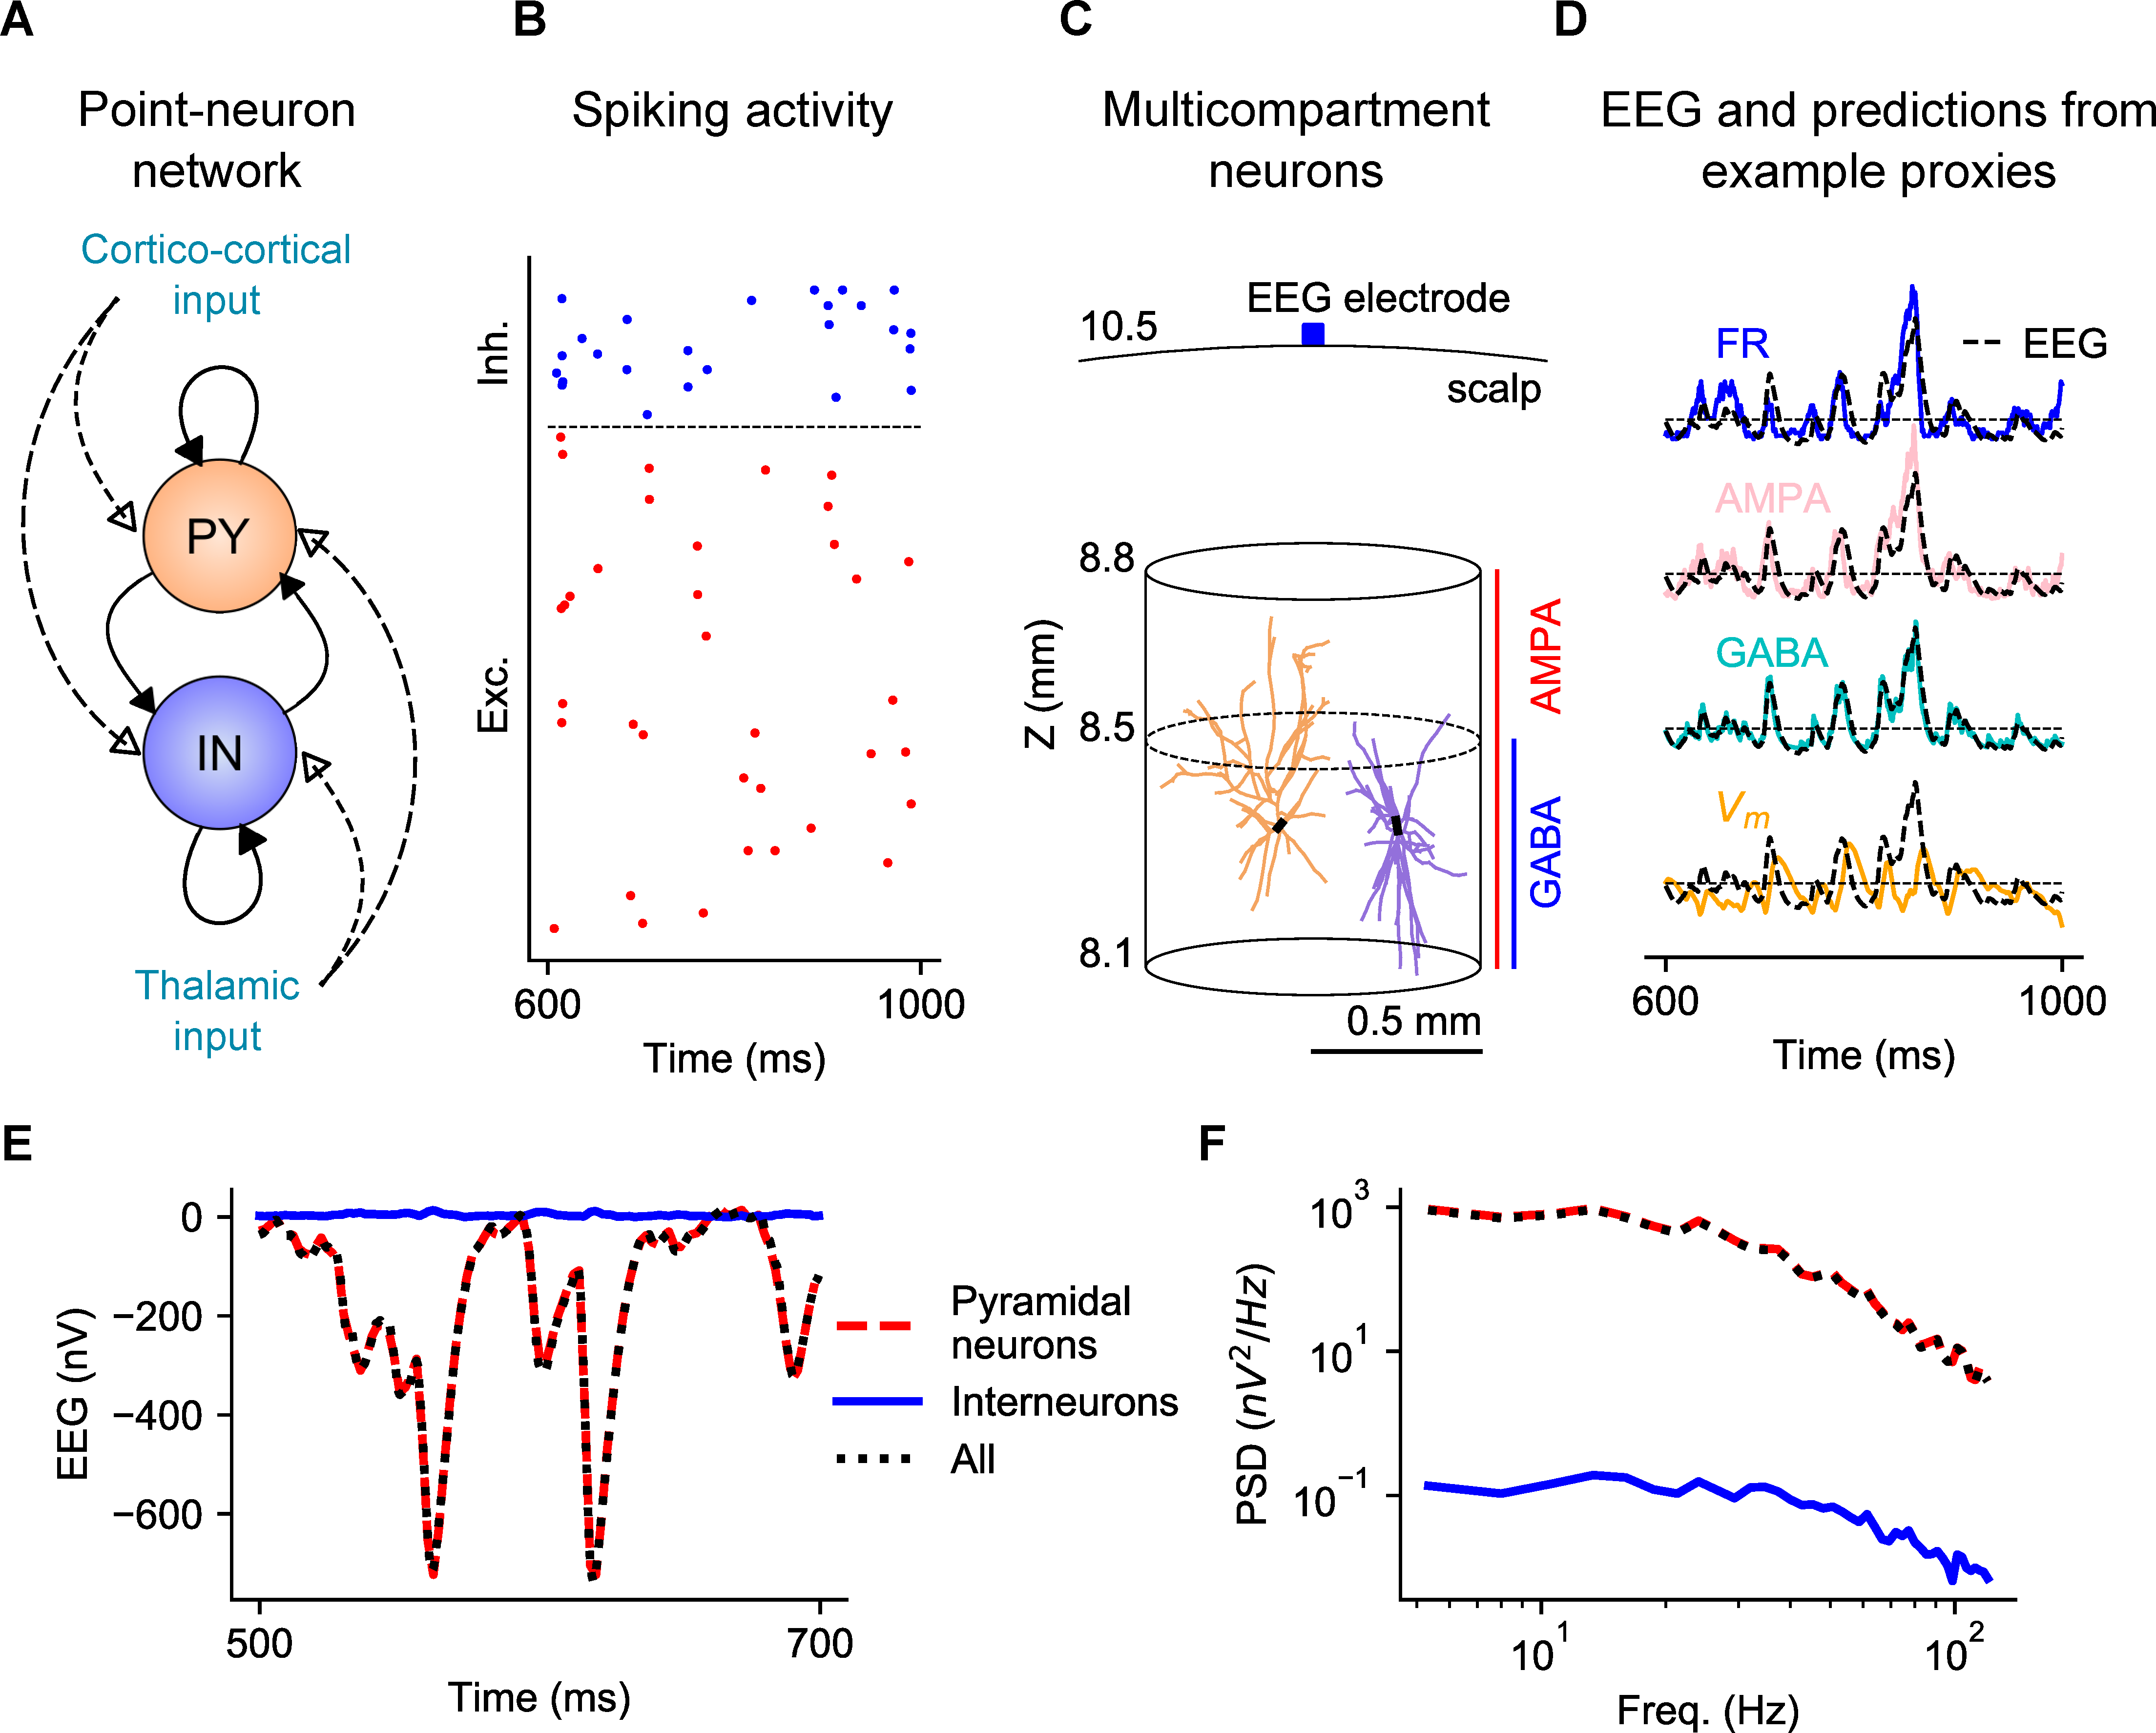
\includegraphics[width=13cm]{Neuronas.png}
	\caption{Descripción general de los modelos de red y cálculo de proxies y EEG de acuerdo con el trabajo realizado en \cite{computationoftheelectroencephalogram}}
    \label{fig:distrnormal}
\end{figure}\

De acuerdo con la proporción de neuronas excitatorias e inhibidoras encontradas en la corteza cerebral, en nuestro modelo $4000$ neuronas son excitatorias (es decir, sus proyecciones sobre otras neuronas forman sinapsis excitadoras similares a AMPA) y $1000$ inhibitorias (es decir, sus proyecciones forman sinapsis similares a GABA), aleatoriamente conectados con una probabilidad de conexión entre cada par de neuronas de $0,2$. Todas las neuronas en el modelo reciben dos entradas externas (tanto una entrada talámica sensorial como una entrada intracortical, que representa ruido cortical) que fueron diseñadas para predecir algunos aspectos clave de la actividad neuronal en la corteza visual primaria durante la estimulación visual naturalista y la actividad espontánea.

Ref. \cite{methodsforinferring}.
Ref. \cite{understanding}

\chapter{Paralelización de las simulaciones en un servidor}\label{part:simulaciones}

La paralelización puede mejorar la eficiencia de la ejecución de simulaciones a gran escala aprovechando máquinas multinúcleo/multiprocesador, clústeres de computadoras o supercomputadoras. En este caso, para las simulaciones se ha utilizado un servidor con sistema operativo Linux que cuenta con $32$ núcleos disponibles y se ha hecho uso de la totalidad de ellos. A su vez, ha estado disponible una memoria RAM de $128$Gb. Y el sistema tiene capacidad para almacenar hasta $2$TB de información.

\begin{figure}[h]
	\centering
	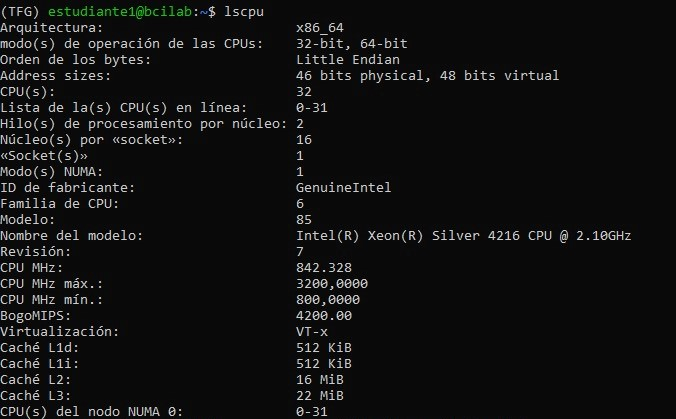
\includegraphics[width=13cm]{CaracteristicasSistema.jpeg}
	\caption{Información del servidor.}
    \label{fig:distrnormal}
\end{figure}\

Gracias a servidor ha sido posible realizar una gran cantidad de simulaciones para disponer del mayor número de datos posibles modificando ciertos parámetros del modelo neuronal que se explicarán a continuación.

Para ejecutar las simulaciones se ha instalado NEST, que es un simulador de red neuronal de spikes utilizado en neurociencia computacional para simular dinámicas de interacción entre neuronas. NEST utiliza de forma nativa OpenMP (\cite{openMP}) para ejecutarse en las computadoras multinúcleo y multiprocesador sin necesidad de bibliotecas adicionales.

En el modelo neuronal utilizado, estamos usando un total de 5000 neuronas de las cuales 4000 son excitatorias y 1000 son inhibitorias. En cada simulación se estudia el comportamiento de estas neuronas y su actividad neuronal en intervalos de 1 ms. Por lo tanto, obtenemos 1000 puntos de actividad neuronal simulada. Sin embargo se ha observado que en los 100 primeros ms aparecían resultados de actividad transitoria que podría afectar la interpretación de los resultados, por lo tanto, para cada una de las simulaciones se ha seleccionado el intervalo de $100$ a $999$ ms.

Para la obtención de de todo el conjunto de datos se han realizado un total de $480$ simulaciones en los cuales se han ido variando cada una de las $5$ variables de la red neuronal que son objeto de estudio de este proyecto.

Cuatro variables se corresponden con las conductancias sinápticas de pico, que determinan la intensidad de las conexiones entre los distintos tipos de neuronas.

\begin{itemize}
    \item Conductancia sináptica de excitatorias a excitatorias (variable exc\_exc\_recurrent).
    \item Conductancia sináptica de excitatorias a inhibitorias (variable exc\_inh\_recurrent).
    \item Conductancia sináptica de inhibitorias a inhibitorias (variable inh\_inh\_recurrent).
    \item Conductancia sináptica de inhibitorias a excitatorias (variable inh\_exc\_recurrent).
\end{itemize}

\begin{figure}[htb]
	\centering
	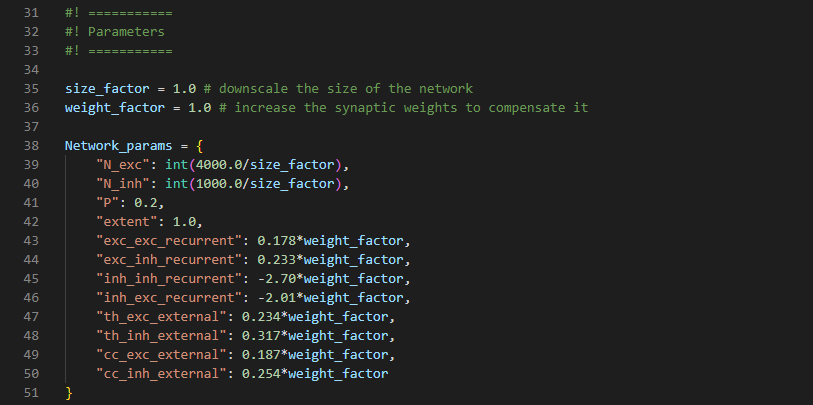
\includegraphics[width=16cm]{Código parámetros.png}
	\caption{Código donde se representan los valores de referencia de las conductancias sinápticas del modelo.}
\end{figure}

La última variable $v_{0}$ que se corresponde con la tasa de entrada externa del modelo, la cual han variado entre dos valores; 1.5 spikes/seg y 2.5 spikes/s. Por lo tanto se han obtenido obtenido 240 simulaciones con el parámetro $v_{0} = 1.5$ y otras 240 simulaciones con el parámetro $v_{0} = 2.5$

\begin{figure}[htb]
	\centering
	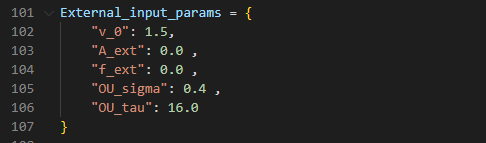
\includegraphics[width=12cm]{Código parámetro v_0.png}
	\caption{Código donde se representan los parámetros que describen la entrada externa del modelo, entre ellos  $v_{0}$ .}
\end{figure}

\section{Análisis de los datos}\label{part:analisis}

En primer lugar hemos estudiado las distintas salidas de actividad neuronal que genera el modelo y como pueden variar según la modificación de los parámetros. Para cada uno de los valores de los parámetros se han repetido las simulaciones 3 veces con el objetivo de promediar la aleatoriedad del modelo (e.g., las conexiones aleatorias entre neuronas).

Para cada una de las simulaciones se obtienen 9 archivos distintos correspondientes a distintas salidas del modelo (e.g., spikes, corrientes sinápticas AMPA y GABA) pero únicamente se han utilizado en este caso, los archivos .AMPA y .GABA que serán útiles para el cálculo del EEG, usando la siguiente fórmula que en trabajos previos ha demostrado aproximar bien el EEG, \cite{computationoftheelectroencephalogram}.

\begin{equation}
    EEG = \abs{AMPA} + \abs{GABA}
\end{equation}

Los archivos .spikes que usaremos para visualización pero no para análisis posterior de resultados.

Se mostrará a continuación las gráficas obtenidas en puntos de relevancia gracias a los cuales va a ser posible observar diferencias notables en cada una de ellas.

\newpage
\subsection{Resultados de una simulación con los parámetros estándar}

En esta simulación los valores de los parámetros de la red neuronal son los valores de referencia del modelo que en trabajos anteriores se ha demostrado que capturan gran parte de la dinámica cortical, \cite{encodigofnaturalistic}.

\begin{itemize}
    \item exc\_exc\_recurrent: 0.178
    \item exc\_inh\_recurrent: 0.233
    \item inh\_inh\_recurrent: -2.70
    \item inh\_exc\_recurrent: -2.01
\end{itemize}

\begin{figure}[htb]
	\centering
	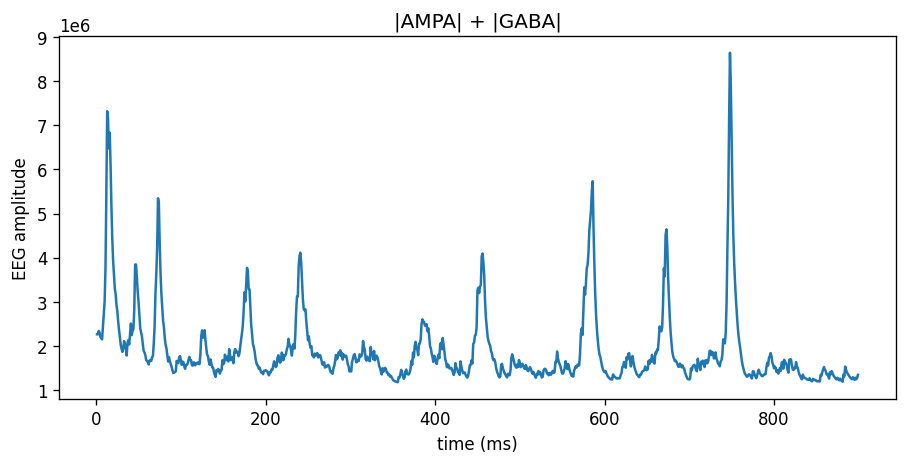
\includegraphics[width=12cm]{EEG-Estandar.png}
	\caption{Gráfica EEG con parámetros estandar.}
\end{figure}

\begin{figure}[htb]
	\centering
	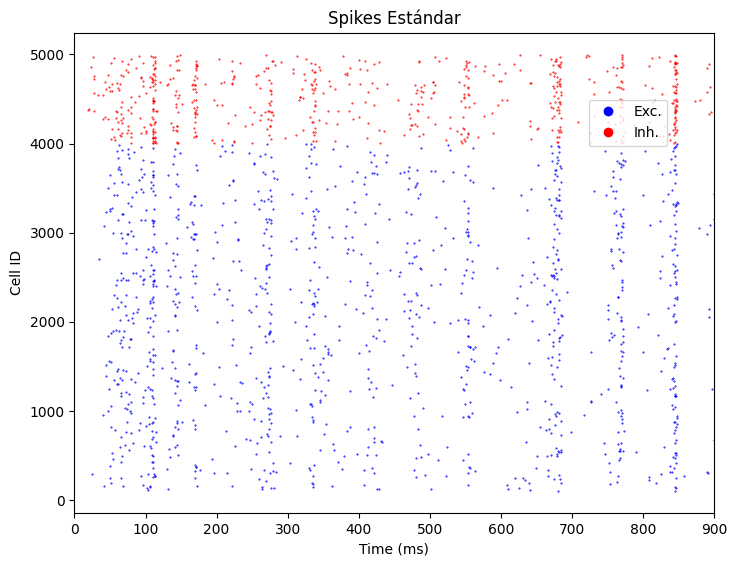
\includegraphics[width=12cm]{Spikes-Estandar.png}
	\caption{Gráfica de spikes con parámetros estandar.}
\end{figure}

\newpage
\subsection{Resultados de una simulación con parámetro exc\_exc\_recurrent alterado (0.005)}

Para esta simulación se ha realizado la ejecución con los valores estándar excepto para la variable exc\_exc\_recurrent que su valor se ha reducido al mínimo (0.005). Se observa una reducción generalizada de la actividad neuronal.

\begin{figure}[htb]
	\centering
	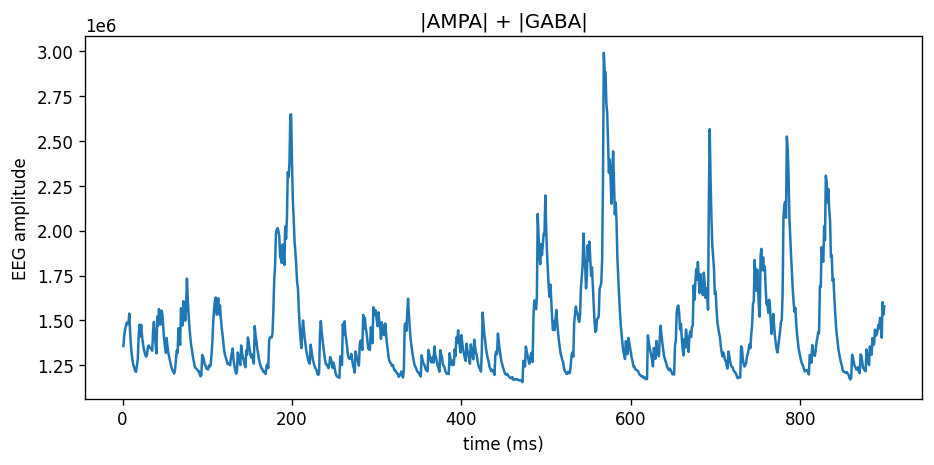
\includegraphics[width=12cm]{EEG-Exc_Exc-0.005.png}
	\caption{Gráfica EEG con parámetro exc\_exc = 0.005.}
\end{figure}

\begin{figure}[htb]
	\centering
	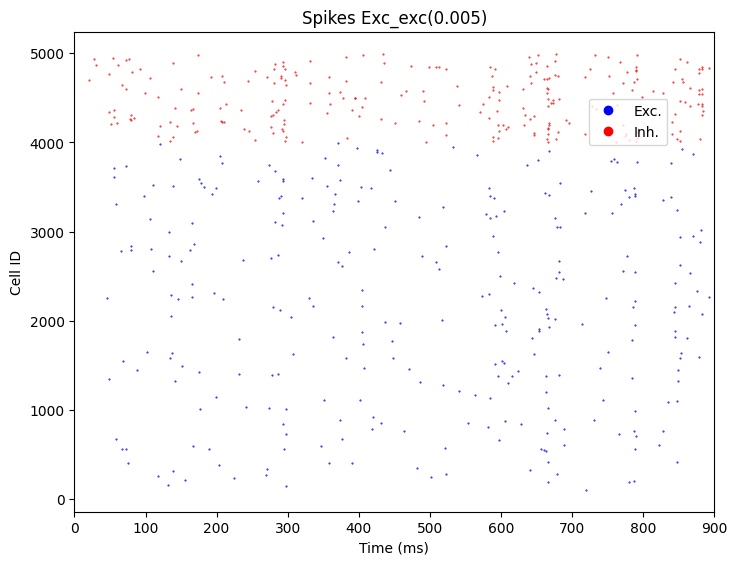
\includegraphics[width=12cm]{Spikes-Exc_Exc-0.005.png}
	\caption{Gráfica de spikes con parámetro exc\_exc = 0.005.}
\end{figure}

\newpage
\subsection{Resultados de una simulación con parámetro exc\_exc\_recurrent alterado (0.200)}

Para esta simulación se ha realizadao la ejecución con los valores estándar excepto para la variable exc\_exc\_recurrent que su valor se ha aumentado levemente con respecto al estándar (0.200). Se observa una leve sincronización que produce oscilaciones periódicas.

\begin{figure}[htb]
	\centering
	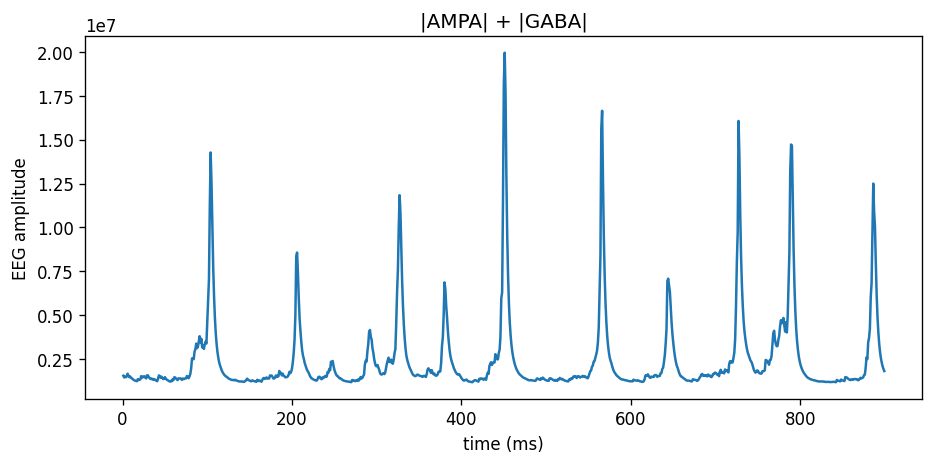
\includegraphics[width=12cm]{EEG-Exc_Exc-0.200.png}
	\caption{Gráfica EEG con parámetro exc\_exc = 0.200.}
\end{figure}

\begin{figure}[htb]
	\centering
	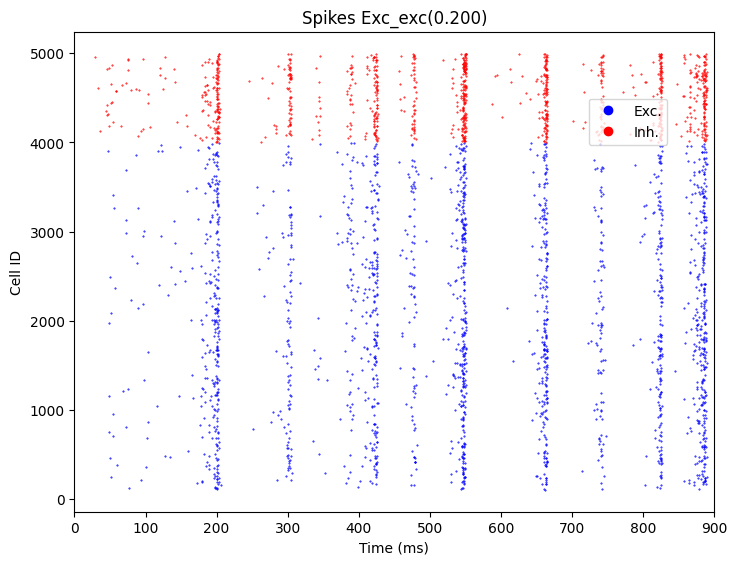
\includegraphics[width=12cm]{Spikes-Exc_Exc-0.200.png}
	\caption{Gráfica de spikes con parámetro exc\_exc = 0.200.}
\end{figure}

\newpage
\subsection{Resultados de una simulación con parámetro exc\_exc\_recurrent alterado (0.450)}

Para esta simulación se ha realizadao la ejecución con los valores estándar excepto para la variable exc\_exc\_recurrent que su valor se ha aumentado considerablemente con respecto al estándar (0.450). Este correspondería con un escenario irrealista de sincronización muy elevada.

\begin{figure}[htb]
	\centering
	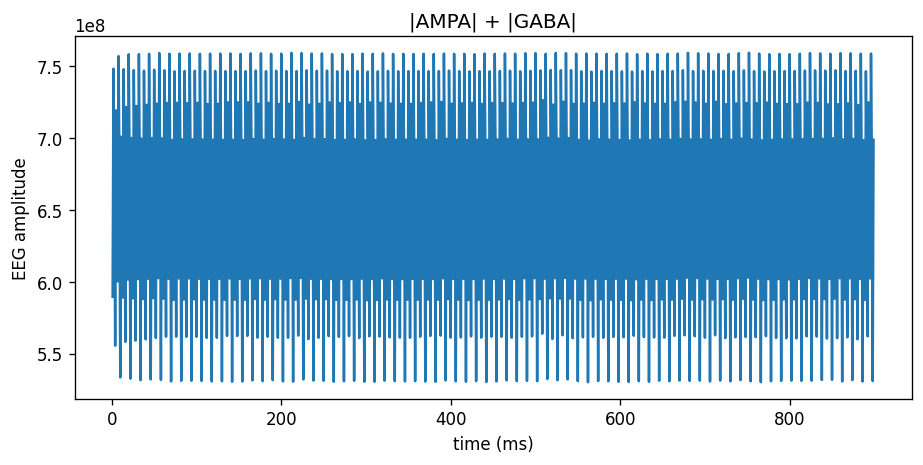
\includegraphics[width=12cm]{EEG-Exc_Exc-0.450.png}
	\caption{Gráfica EEG con parámetro exc\_exc = 0.450.}
\end{figure}

\begin{figure}[htb]
	\centering
	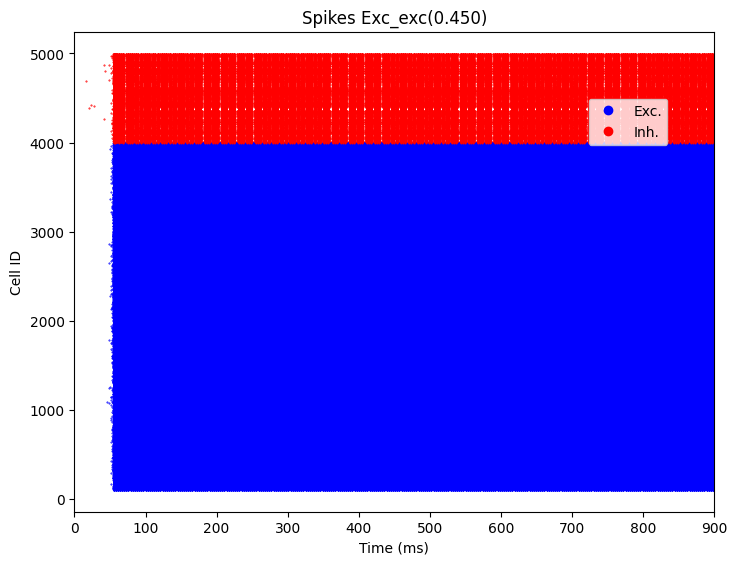
\includegraphics[width=12cm]{Spikes-Exc_Exc-0.450.png}
	\caption{Gráfica de spikes con parámetro exc\_exc = 0.450.}
\end{figure}

\newpage
\subsection{Resultados de una simulación con parámetro inh\_exc\_recurrent alterado (-0.25)}

Para esta simulación se ha realizado la ejecución con los valores estándar excepto para la variable inh\_exc\_recurrent que su valor se ha aumentado considerablemente con respecto al estándar (-0.25). De nuevo observamos una respuesta demasiado sincronizada.

\begin{figure}[htb]
	\centering
	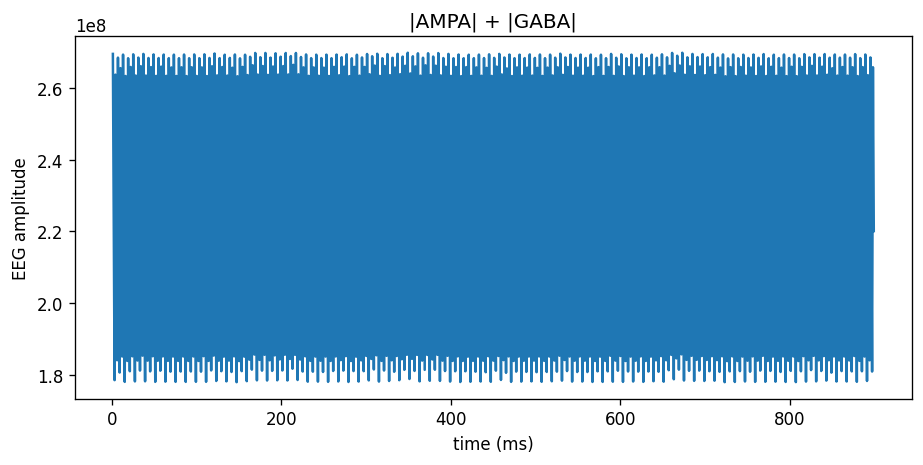
\includegraphics[width=12cm]{EEG-Inh_Exc--0.25.png}
	\caption{Gráfica EEG con parámetro inh\_exc = -0.25.}
\end{figure}

\begin{figure}[htb]
	\centering
	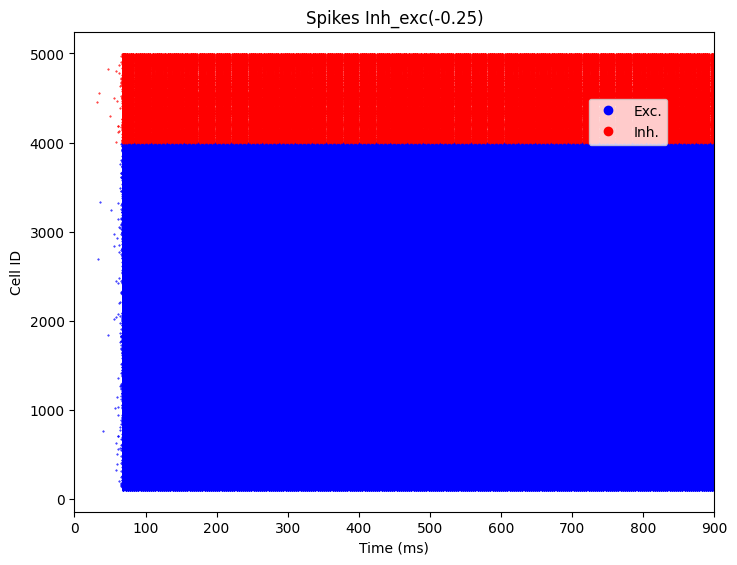
\includegraphics[width=12cm]{Spikes-Inh_Exc--0.25.png}
	\caption{Gráfica de spikes con parámetro inh\_exc = -0.25.}
\end{figure}

\newpage
\subsection{Resultados de una simulación con parámetro inh\_exc\_recurrent alterado (-4.50)}

Para esta simulación se ha realizadao la ejecución con los valores estándar excepto para la variable inh\_exc\_recurrent que su valor se ha disminuido considerablemente con respecto al estándar (-4.50). La red produce una salida muy atenuada.

\begin{figure}[htb]
	\centering
	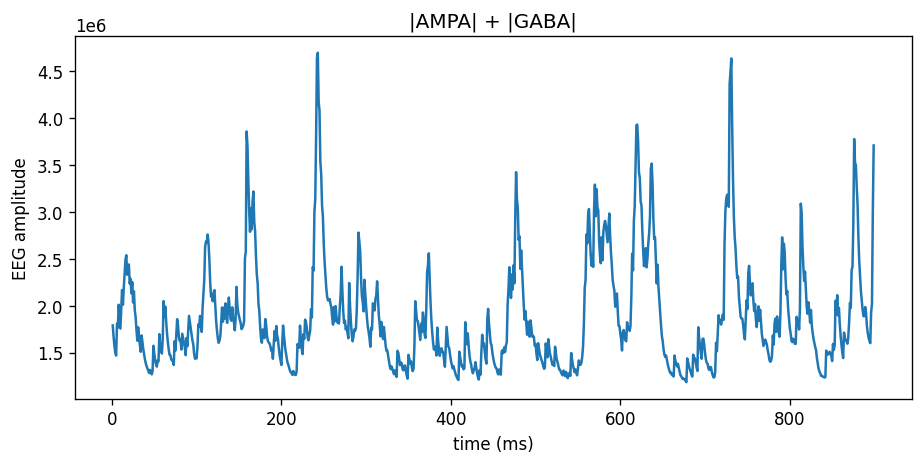
\includegraphics[width=12cm]{EEG-Inh_Exc--4.50.png}
	\caption{Gráfica EEG con parámetro inh\_exc = -4.50.}
\end{figure}

\begin{figure}[htb]
	\centering
	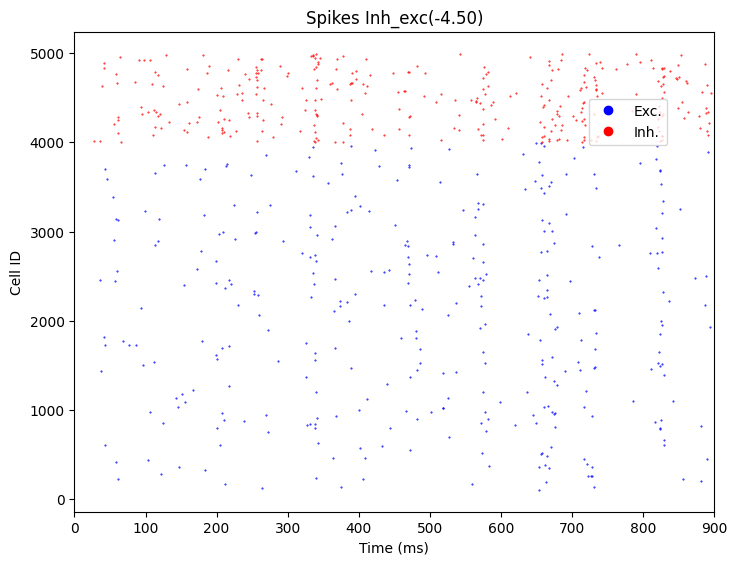
\includegraphics[width=12cm]{Spikes-Inh_Exc--4.50.png}
	\caption{Gráfica de spikes con parámetro inh\_exc = -4.50.}
\end{figure}\


\newpage
\subsection{Resultados de una simulación con parámetro inh\_exc\_recurrent alterado (-8.00)}

Para esta simulación se ha realizadao la ejecución con los valores estándar excepto para la variable inh\_exc\_recurrent que su valor se ha disminuido al mínimo con respecto al estándar (-8.00). A penas se diferencian puntos en los cuales se produzcan reacciones neuronales sincronizadas.

\begin{figure}[htb]
	\centering
	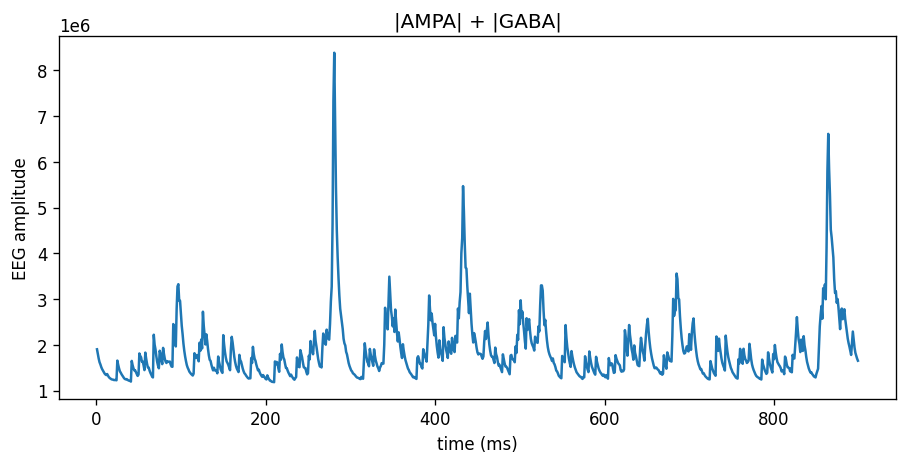
\includegraphics[width=12cm]{EEG-Inh_Exc--8.00.png}
	\caption{Gráfica EEG con parámetro inh\_exc = -8.00.}
\end{figure}

\begin{figure}[htb]
	\centering
	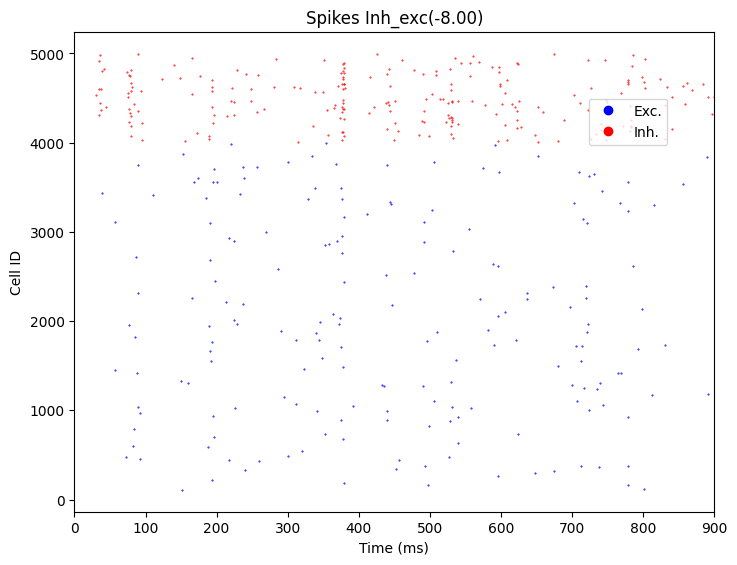
\includegraphics[width=12cm]{Spikes-Inh_Exc--8.00.png}
	\caption{Gráfica de spikes con parámetro inh\_exc = -8.00.}
\end{figure}\

\newpage

\chapter{Conclusiones del análisis de los datos}

A partir del estudio de este tipo de gráficas, se pueden observar distintos tipos de comportamientos que en determinados casos se pueden asociar con resultados de cerebros de personas humanas que sufren algún tipo de enfermedad relacionada con el sistema nervioso. Un ejemplo de gráficas similares a las obtenida en las figura 6 y 16 podría ser la de una persona diagnosticada con trastorno del espectro autista (TEA) ya que a penas se diferencian puntos en los cuales se observan una gran actividad neuronal. 

Esta información, además del estudio de anomalías genéticas, conduce a un modelo que postula que algunas formas de autismo son causadas por una mayor proporción de excitación/inhibición en los sistemas sensorial, mnemotécnico, social y emocional. El modelo postula además que el aumento de la proporción de excitación/inhibición puede ser causado por efectos combinatorios de variables genéticas y ambientales que inciden sobre un sistema neuronal dado, se ha estudiado en profundidad en \cite{modelofautism}.

\newpage
\chapter{Estimación de parámetros del circuito neuronal a partir de la señal del encefalograma}\label{part:estimaciones}

Uno de los objetivos de la realización de este proyecto es la estimación de parámetros del circuito neuronal a partir de la señal del encefalograma. Para ello, se ha programado en Python varios algoritmos de Machine Learning gracias a la librería sklearn obteniendo distintos resultados.

Los datos sobre los que se han trabajado han sido las 3 repeticiones de las simulaciones en las que se ha variado el valor de la variable exc\_exc e inh\_exc combinadas con los dos valores del parámetro $v_{0}$. Se han almacenado los valores del EEG en una variable $X$ en la que en cada elemento tenemos un vector con todos los valores del EGG de esa simulación y otra variable $Y$ multidimensional que se corresponden con los valores de los ratios de conductancias $g$ calculados como:

\begin{equation}
    g = \frac{g\_exc}{g\_inh}
\end{equation}

y con con los valores de la tasa de entrada del tálamo $v_0$.

\begin{figure}[H]
	\centering
	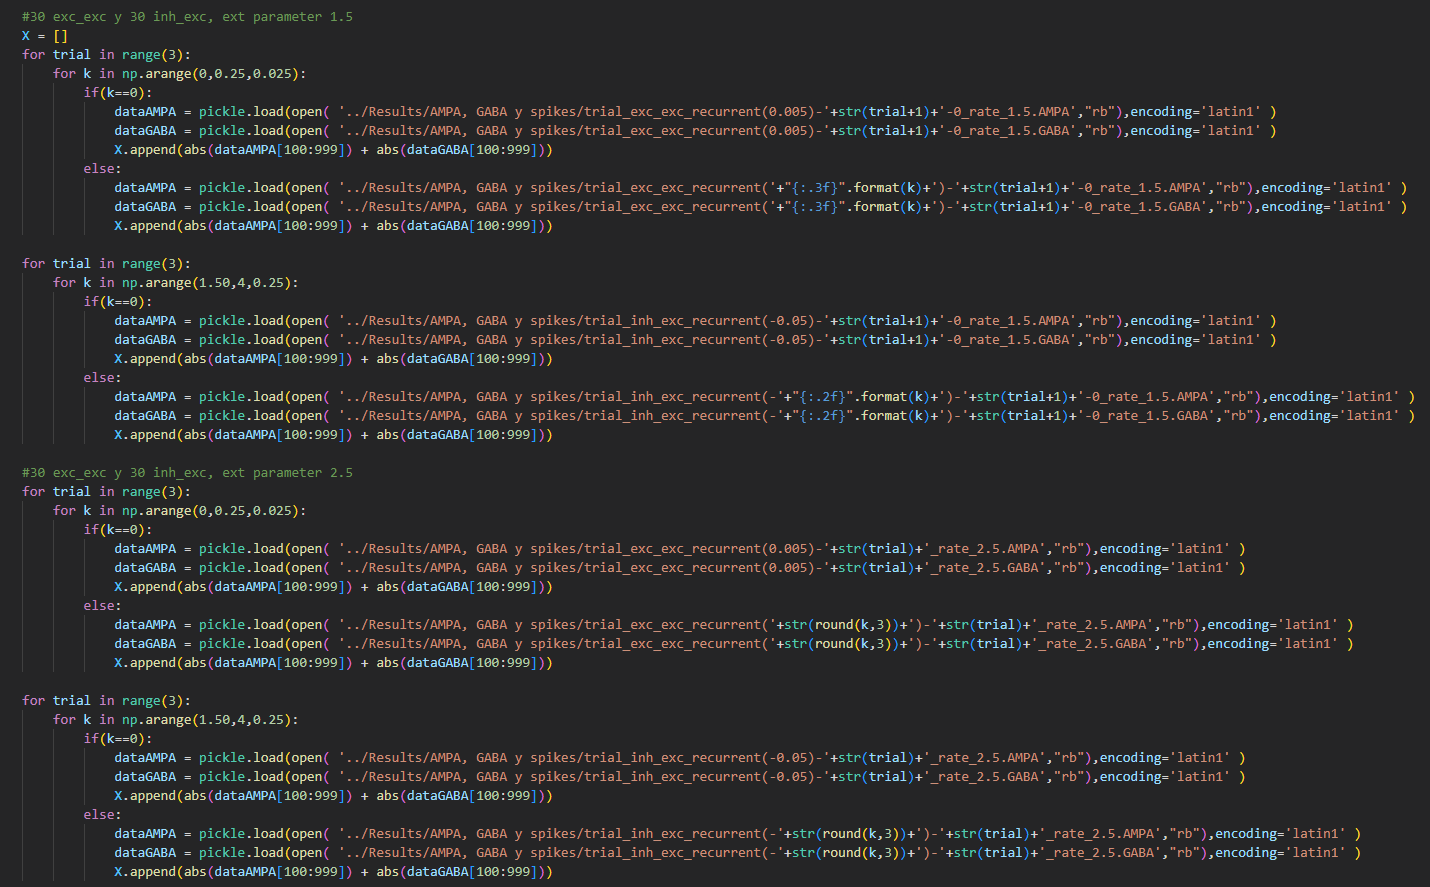
\includegraphics[width=17cm]{Fuente de datos variable X.png}
	\caption{Fuente de datos variable X}
\end{figure}

Antes de entrenar cada uno de los modelos se han normalizado haciendo uso de las herramientas de preprocesamiento proporcionadas por la librería sklearn. Además de dividir los datos entre datos de entrenamiento y datos de test para poder evaluar posteriormente mediante cross-validation cada uno de los modelos. Para ello elegimos el ochenta por ciento de datos como entrenamiento y el veinte por ciento restante para test.

A continuación, veremos los resultados obtenidos en forma de gráficas después de utilizar cada uno de los diferentes algoritmos.


\section{Algoritmo de regresión lineal simple}

La regresión lineal simple es un método que usa la relación estadística entre dos variables cuantitativas en la que una variable, la variable de respuesta (o variable dependiente) puede ser predicha a partir de otra variable (la variable predictora o independiente). 

A continuación, se muestra el código utilizado para obtener el resultado de los errores cuadráticos medios después de $1000$ ejecuciones para evitar aleatoriedad. Donde podemos diferenciar varias partes:\\
- Creación de los datos de entrenamiento y de tests.\\
- Escalado de entrada para ajustar los datos al modelo.\\
- Entrenamiento del modelo donde se llama a algoritmo de regresión lineal.\\
- Evaluación del modelo haciendo uso de los errores cuadráticos medios.

\begin{figure}[H]
	\centering
	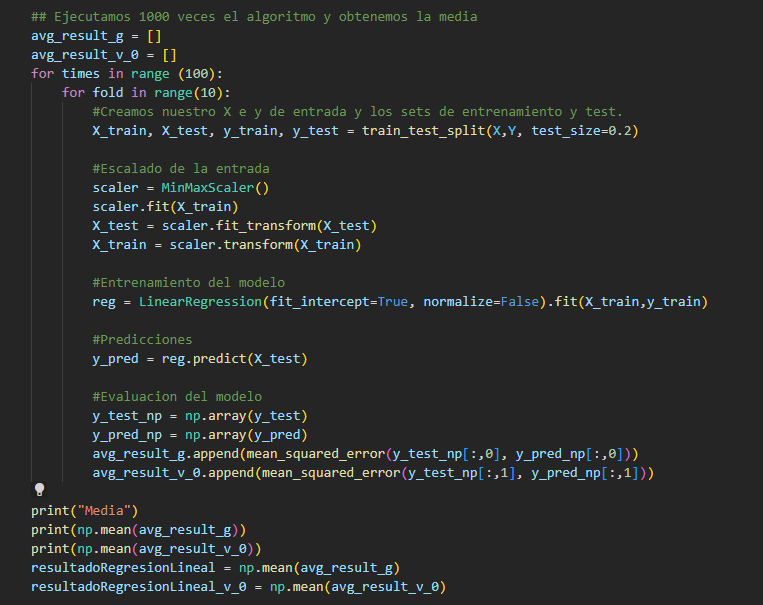
\includegraphics[width=15cm]{Código algoritmo lineal simple.png}
\end{figure}

\subsection{Machine Learning con algoritmo de regresión lineal simple}

\begin{figure}[H]
	\centering
	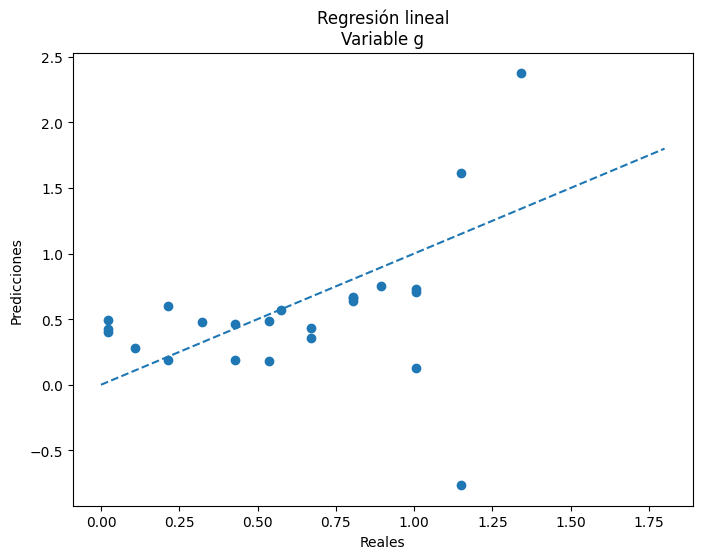
\includegraphics[width=11cm]{Regresión lineal Variable g.png}
\end{figure}

\begin{figure}[H]
	\centering
	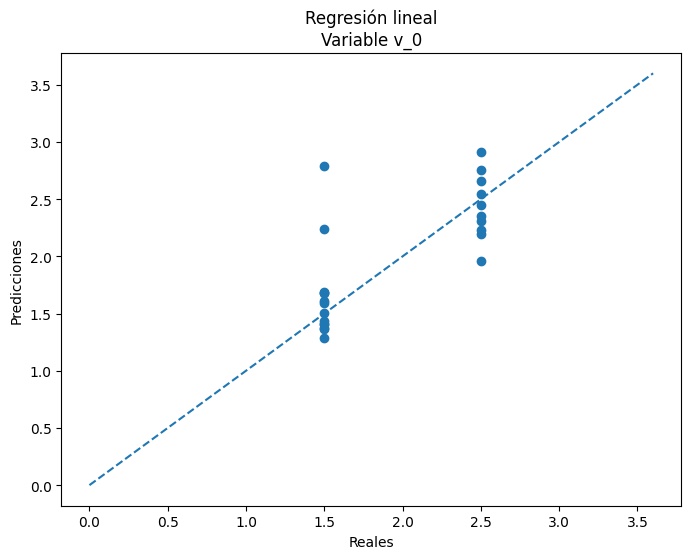
\includegraphics[width=11cm]{Regresión lineal Variable v_0.png}
\end{figure}

\subsection{Machine Learning con algoritmo de regresión lineal simple aplicando autocorrelación}

\begin{figure}[H]
	\centering
	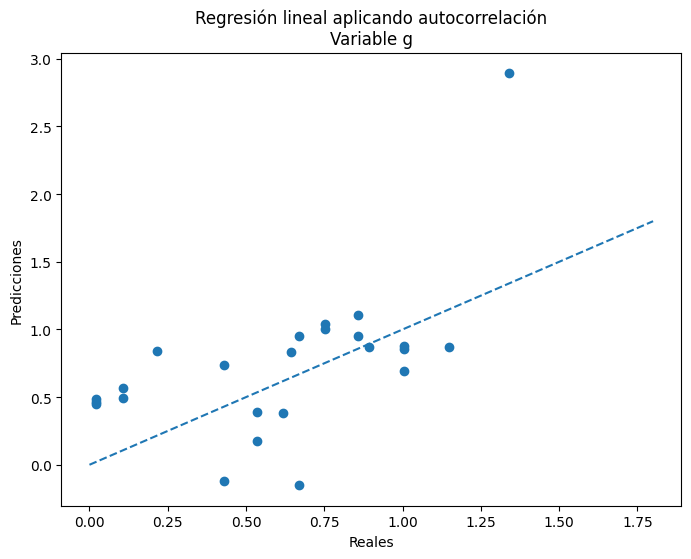
\includegraphics[width=11cm]{Regresión lineal aplicando autocorrelación Variable g.png}
\end{figure}

\begin{figure}[H]
	\centering
	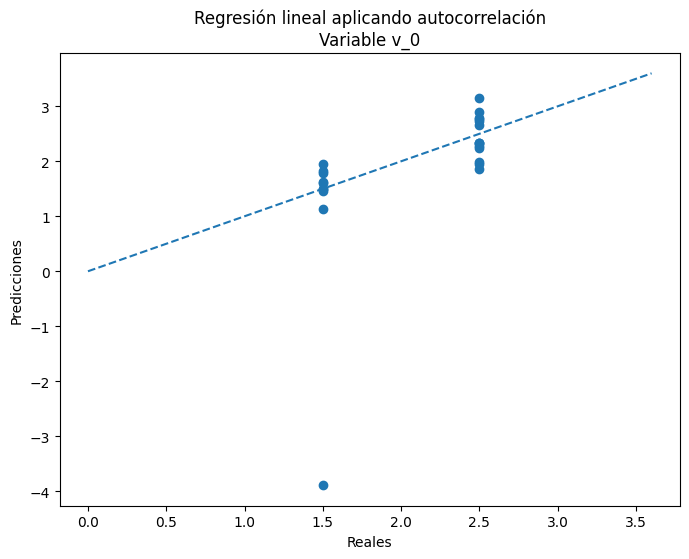
\includegraphics[width=11cm]{Regresión lineal aplicando autocorrelación Variable v_0.png}
\end{figure}

\section{Algoritmo de regresión lineal de Ridge}

La regularización Ridge penaliza la suma de los coeficientes elevados al cuadrado. A esta penalización se le conoce como L2 y tiene el efecto de reducir de forma proporcional el valor de todos los coeficientes del modelo pero sin que estos lleguen a cero. El grado de penalización está controlado por lambda. Cuando lambda=0, la penalización es nula y el resultado es equivalente al de un modelo lineal por mínimos cuadrados ordinarios (OLS). A medida que lambda aumenta, mayor es la penalización y menor el valor de los predictores.

A continuación, se muestra el código utilizado para obtener el resultado de los errores cuadráticos medios después de $1000$ ejecuciones para evitar aleatoriedad. Donde podemos diferenciar varias partes:\\
- Creación de los datos de entrenamiento y de tests.\\
- Escalado de entrada para ajustar los datos al modelo.\\
- Entrenamiento del modelo donde se llama a algoritmo de regresión de Ridge y se va variando alfa.\\
- Evaluación del modelo haciendo uso de los errores cuadráticos medios.

\begin{figure}[H]
	\centering
	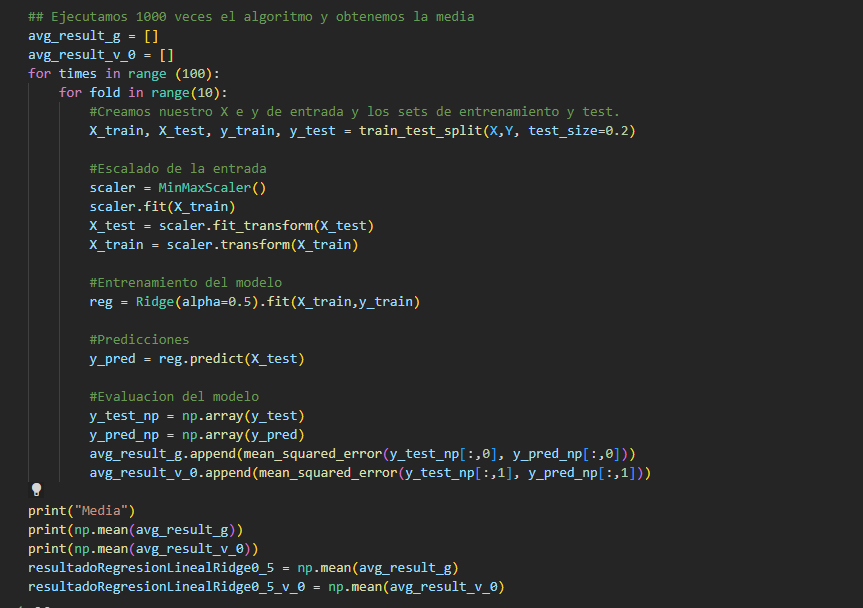
\includegraphics[width=15cm]{Código algoritmo de Ridge.png}
\end{figure}

\subsection{Machine Learning con algoritmo de regresión lineal de Ridge con alfa = 0.5}

\begin{figure}[H]
	\centering
	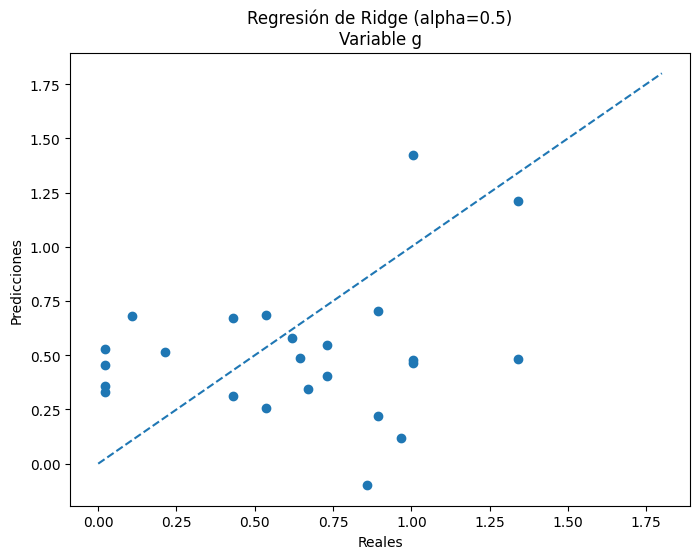
\includegraphics[width=11cm]{Regresión de Ridge (alpha=0.5) Variable g.png}
\end{figure}

\begin{figure}[H]
	\centering
	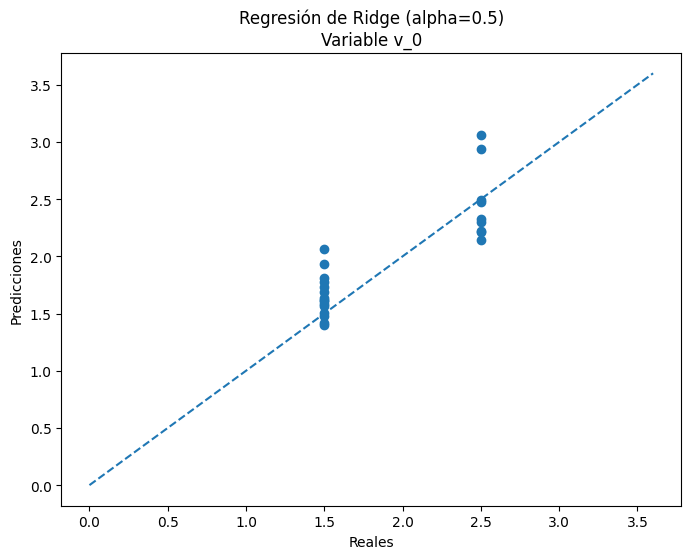
\includegraphics[width=11cm]{Regresión de Ridge (alpha=0.5) Variable v_0.png}
\end{figure}

\subsection{Machine Learning con algoritmo de regresión lineal de Ridge con alfa = 0.5 aplicando autocorrelación}

\begin{figure}[H]
	\centering
	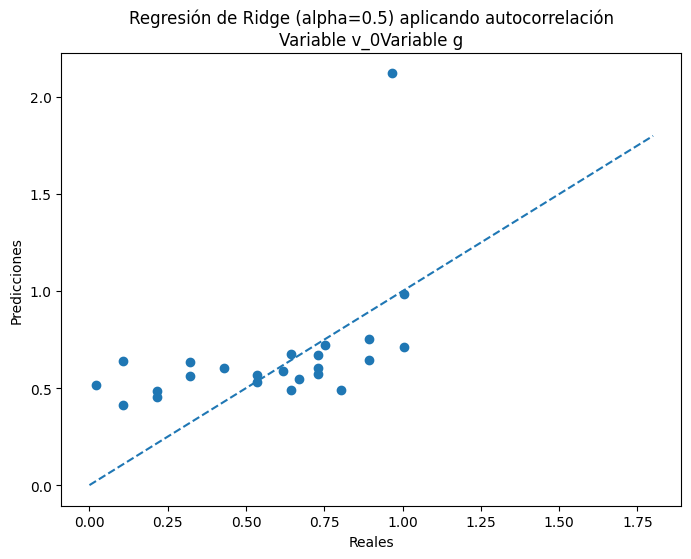
\includegraphics[width=11cm]{Regresión de Ridge (alpha=0.5) aplicando autocorrelación Variable g.png}
\end{figure}

\begin{figure}[H]
	\centering
	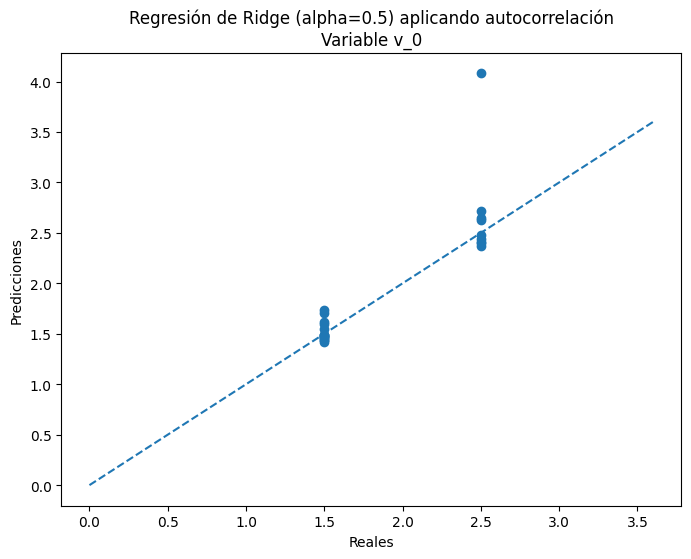
\includegraphics[width=12cm]{Regresión de Ridge (alpha=0.5) aplicando autocorrelación Variable v_0.png}
\end{figure}

\subsection{Machine Learning con algoritmo de regresión lineal de Ridge con alfa = 1}

\begin{figure}[H]
	\centering
	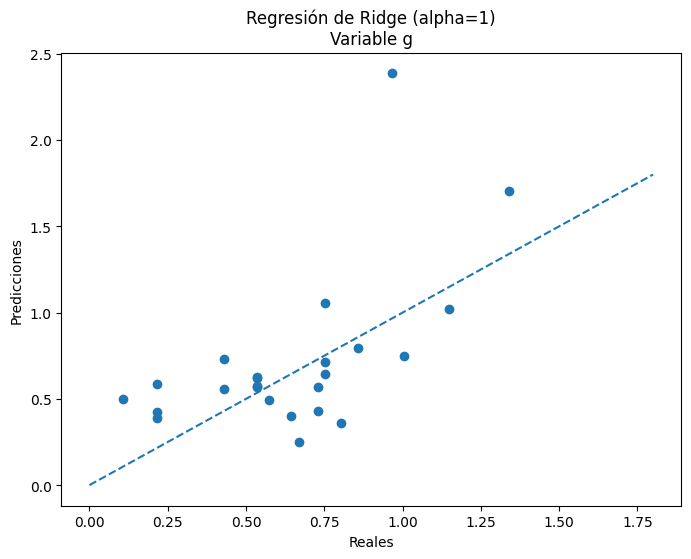
\includegraphics[width=11cm]{Regresión de Ridge (alpha=1) Variable g.png}
\end{figure}

\begin{figure}[H]
	\centering
	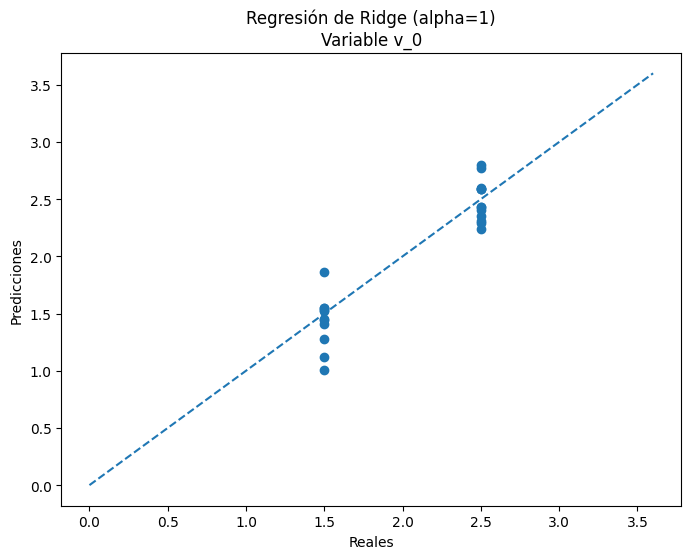
\includegraphics[width=11cm]{Regresión de Ridge (alpha=1) Variable v_0.png}
\end{figure}

\subsection{Machine Learning con algoritmo de regresión lineal de Ridge con alfa = 1 aplicando autocorrelación}

\begin{figure}[H]
	\centering
	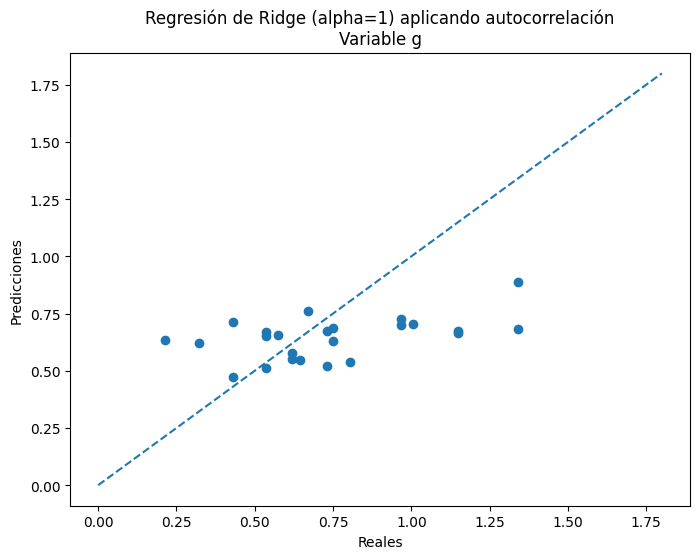
\includegraphics[width=11cm]{Regresión de Ridge (alpha=1) aplicando autocorrelación Variable g.png}
\end{figure}

\begin{figure}[H]
	\centering
	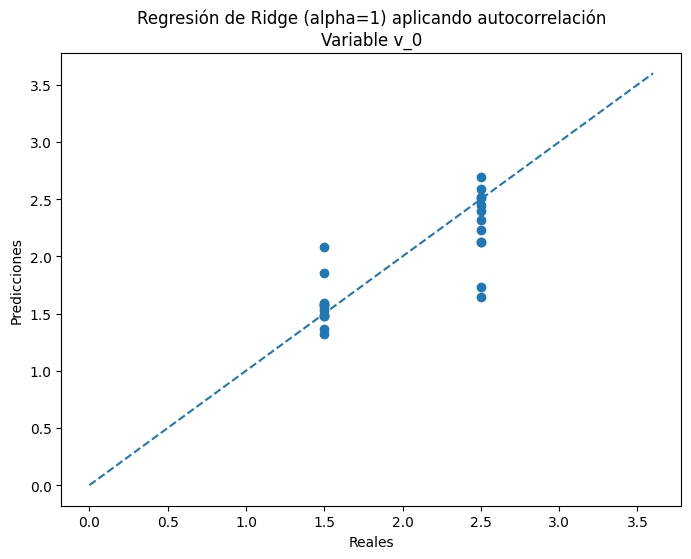
\includegraphics[width=12cm]{Regresión de Ridge (alpha=1) aplicando autocorrelación Variable v_0.png}
\end{figure}

\subsection{Machine Learning con algoritmo de regresión lineal de Ridge con alfa = 1.5}

\begin{figure}[H]
	\centering
	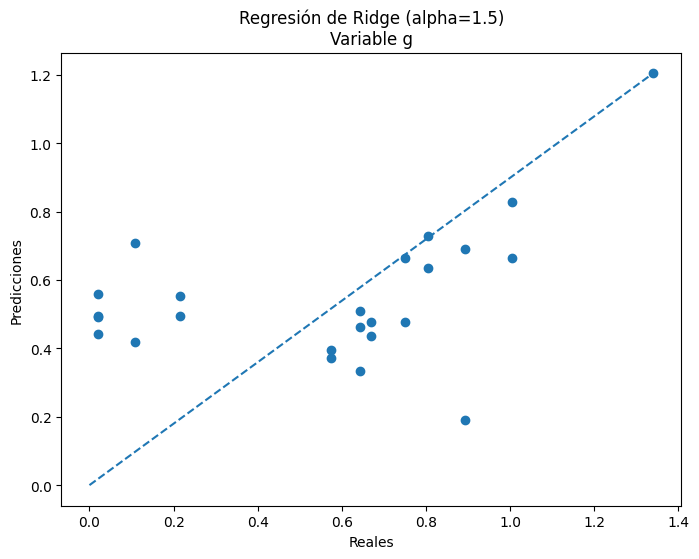
\includegraphics[width=11cm]{Regresión de Ridge (alpha=1.5) Variable g.png}
\end{figure}

\begin{figure}[H]
	\centering
	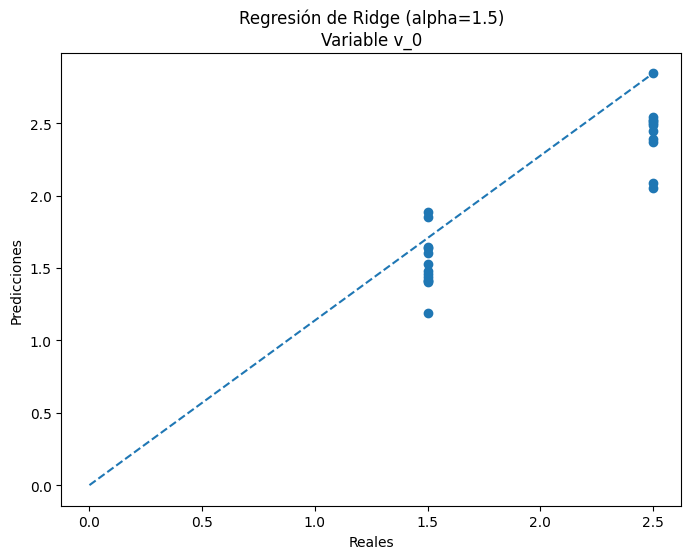
\includegraphics[width=11cm]{Regresión de Ridge (alpha=1.5) Variable v_0.png}
\end{figure}

\subsection{Machine Learning con algoritmo de regresión lineal de Ridge con alfa = 1.5 aplicando autocorrelación}

\begin{figure}[H]
	\centering
	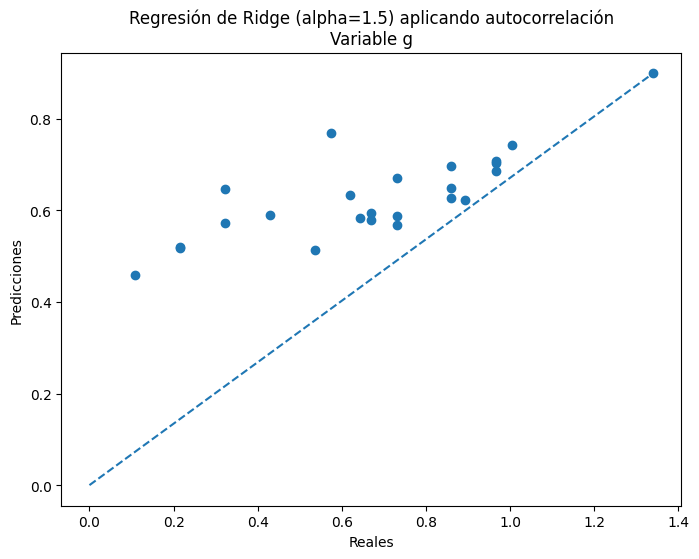
\includegraphics[width=11cm]{Regresión de Ridge (alpha=1.5) aplicando autocorrelación Variable g.png}
\end{figure}

\begin{figure}[H]
	\centering
	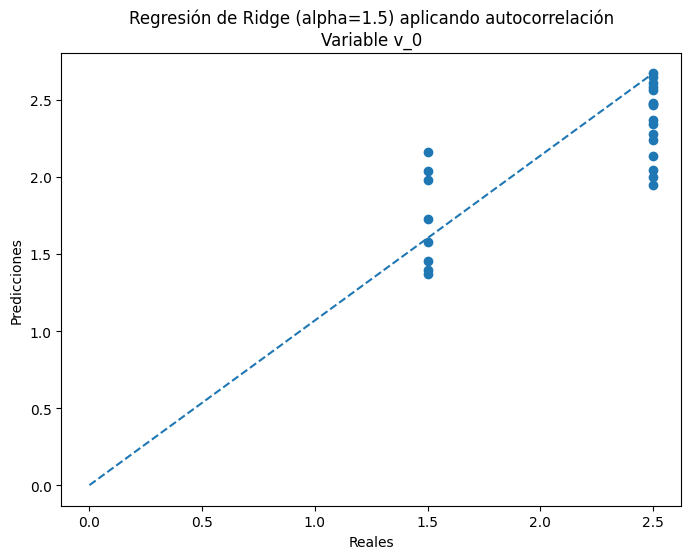
\includegraphics[width=12cm]{Regresión de Ridge (alpha=1.5) aplicando autocorrelación Variable v_0.png}
\end{figure}

\subsection{Machine Learning con algoritmo de regresión lineal de Ridge con alfa = 2}

\begin{figure}[H]
	\centering
	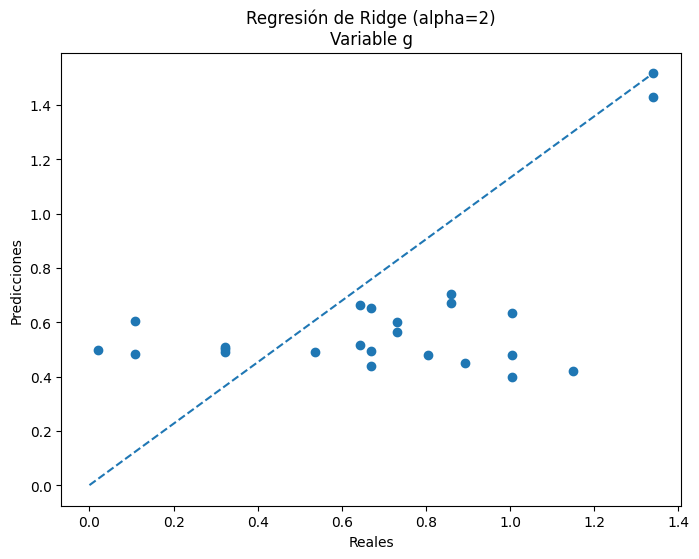
\includegraphics[width=11cm]{Regresión de Ridge (alpha=2) Variable g.png}
\end{figure}

\begin{figure}[H]
	\centering
	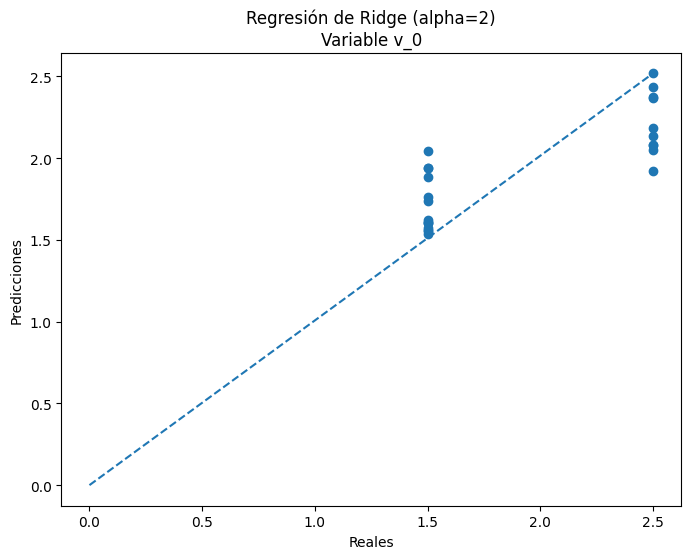
\includegraphics[width=11cm]{Regresión de Ridge (alpha=2) Variable v_0.png}
\end{figure}

\subsection{Machine Learning con algoritmo de regresión lineal de Ridge con alfa = 2 aplicando autocorrelación}

\begin{figure}[H]
	\centering
	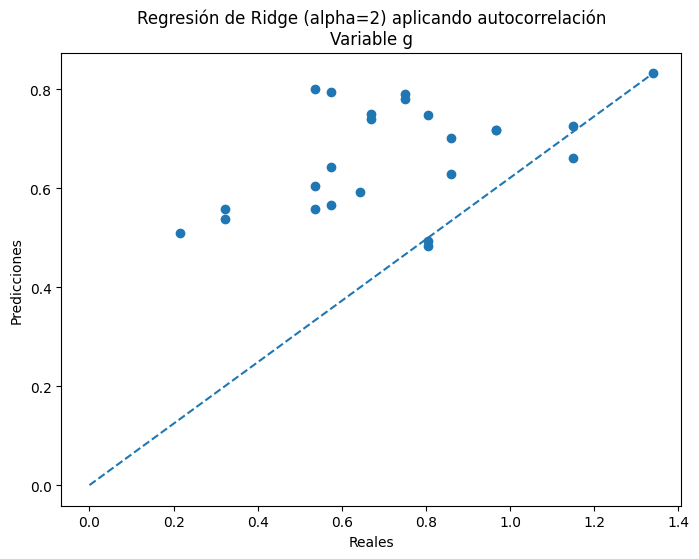
\includegraphics[width=11cm]{Regresión de Ridge (alpha=2) aplicando autocorrelación Variable g.png}
\end{figure}

\begin{figure}[H]
	\centering
	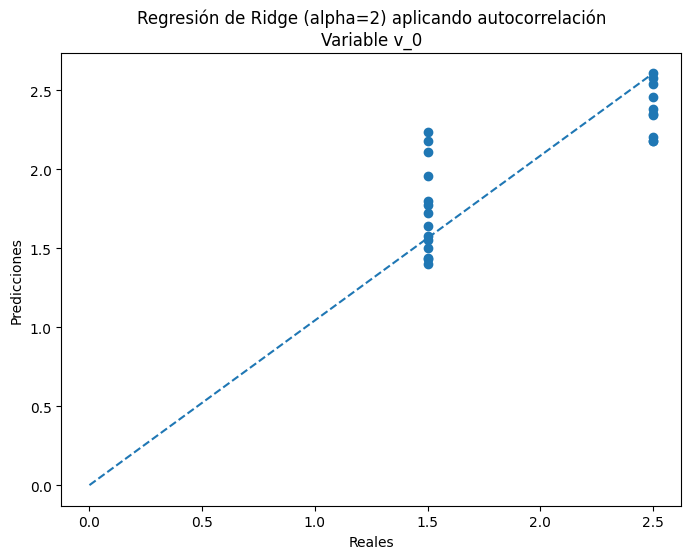
\includegraphics[width=12cm]{Regresión de Ridge (alpha=2) aplicando autocorrelación Variable v_0.png}
\end{figure}

\subsection{Evolución de los resultados variando alfa para regresión lineal de Ridge}

\begin{figure}[H]
	\centering
	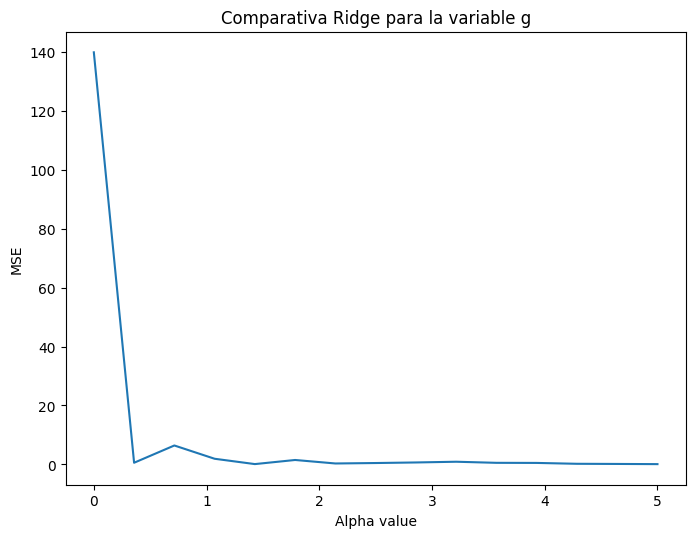
\includegraphics[width=11cm]{Comparativa Ridge para la variable g.png}
\end{figure}

\begin{figure}[H]
	\centering
	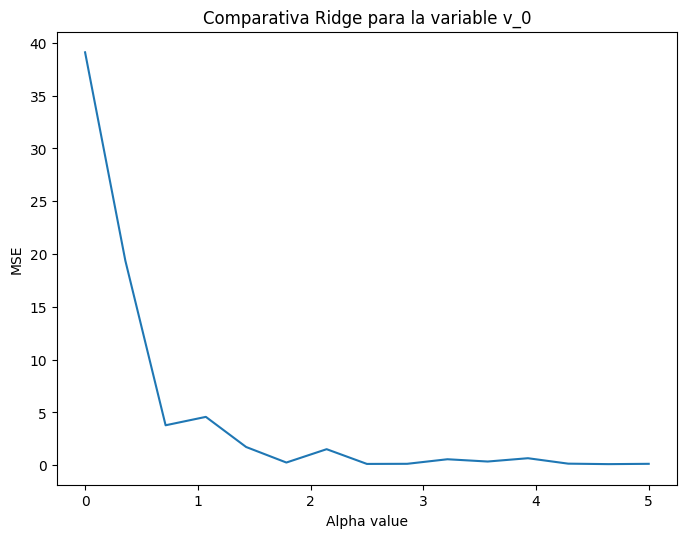
\includegraphics[width=12cm]{Comparativa Ridge para la variable v_0.png}
\end{figure}

Como vemos en ambas gráficas cuando el valor de alfa es cero o cercano a cero, obtenemos un resultado parecido al de la regresión lineal simple, sin embargo, a medida que aumentamos el valor de alfa vamos obteniendo mejores resultados que estabilizan a partir de valores cercanos al $0.5$.

\section{Machine Learning con algoritmos no lineales}

\subsection{Machine Learning con algoritmo no lineal de K-Nearest neightbour}

A continuación, se muestra el código utilizado para obtener el resultado de los errores cuadráticos medios después de $1000$ ejecuciones para evitar aleatoriedad. Donde podemos diferenciar varias partes:

- Creación de los datos de entrenamiento y de tests.\\
- Escalado de entrada para ajustar los datos al modelo.\\
- Entrenamiento del modelo donde se llama a algoritmo de regresión de K-NNeighbors, en este caso con 7 vecinos.\\
- Evaluación del modelo haciendo uso de los errores cuadráticos medios.

\begin{figure}[H]
	\centering
	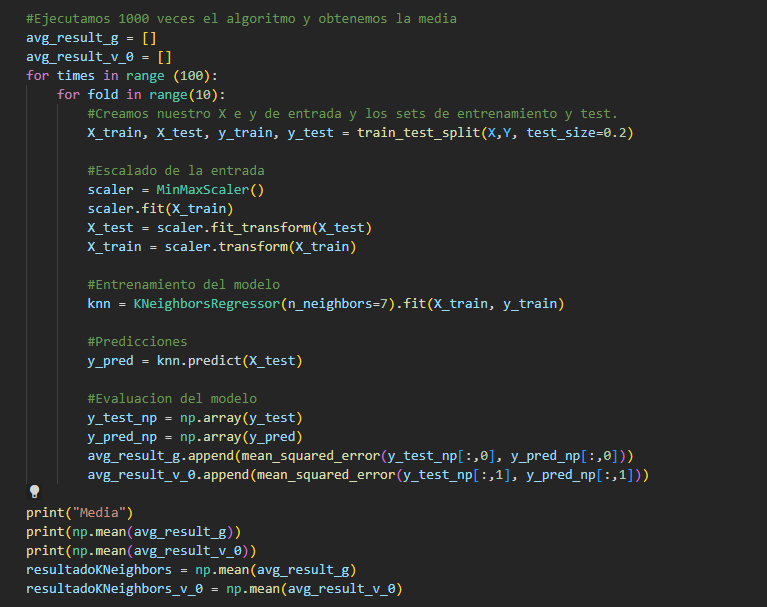
\includegraphics[width=15cm]{Código de K-NNeighbors.png}
\end{figure}

\begin{figure}[H]
	\centering
	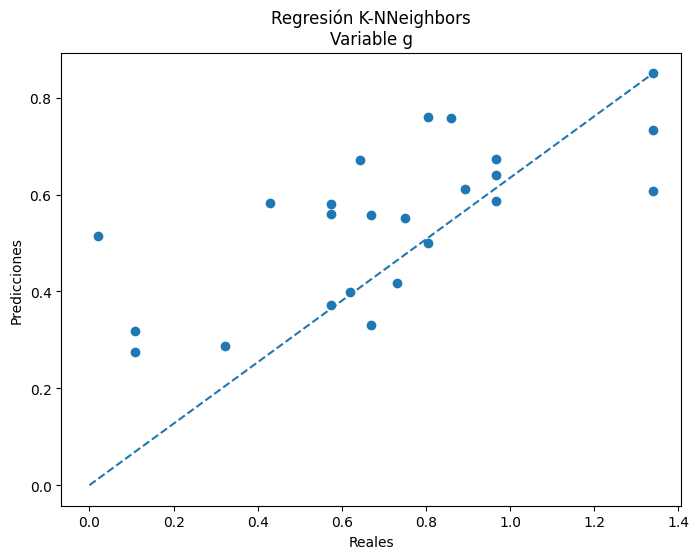
\includegraphics[width=11cm]{Regresión K-NNeighbors Variable g.png}
\end{figure}

\begin{figure}[H]
	\centering
	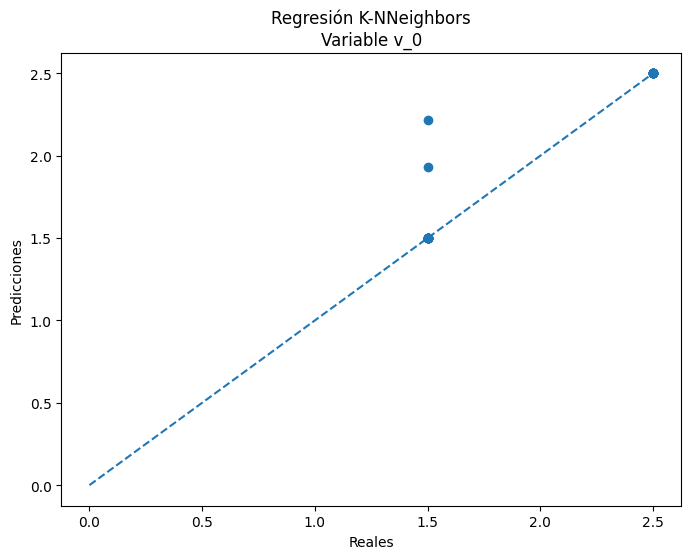
\includegraphics[width=12cm]{Regresión K-NNeighbors Variable v_0.png}
\end{figure}

\subsection{Machine Learning con algoritmo no lineal de K-Nearest neightbour aplicando autocorrelación}

\begin{figure}[H]
	\centering
	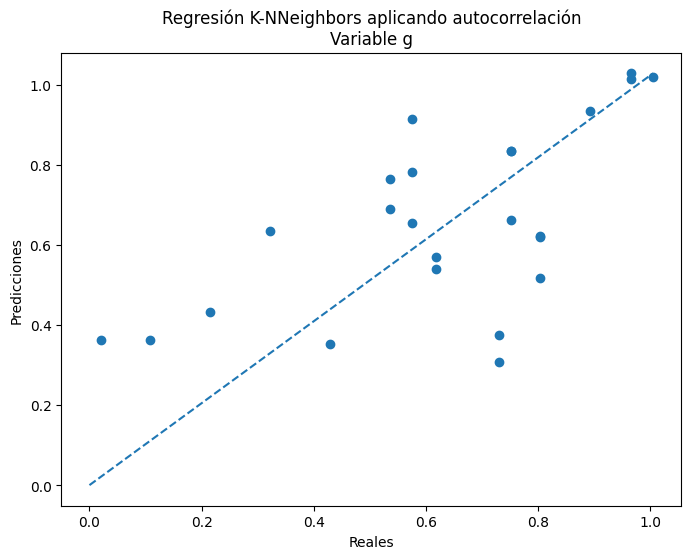
\includegraphics[width=11cm]{Regresión K-NNeighbors aplicando autocorrelación Variable g.png}
\end{figure}

\begin{figure}[H]
	\centering
	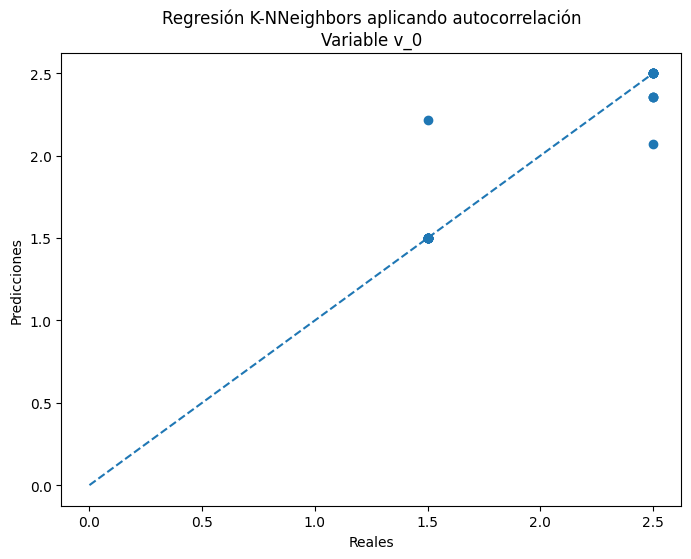
\includegraphics[width=12cm]{Regresión K-NNeighbors aplicando autocorrelación Variable v_0.png}
\end{figure}

\subsection{Machine Learning con algoritmo no lineal - red neuronal}

A continuación, se muestra el código utilizado para obtener el resultado de los errores cuadráticos medios después de $1000$ ejecuciones para evitar aleatoriedad. Donde podemos diferenciar varias partes:\\
- Creación de los datos de entrenamiento y de tests.\\
- Escalado de entrada para ajustar los datos al modelo.\\
- Entrenamiento del modelo donde se llama a la función baseline\_model que se mostrará también a continuación y se han utilizadado como parámetros 100 unidades y 2 capas de profundidad.\\
- Evaluación del modelo haciendo uso de los errores cuadráticos medios.

\begin{figure}[H]
	\centering
	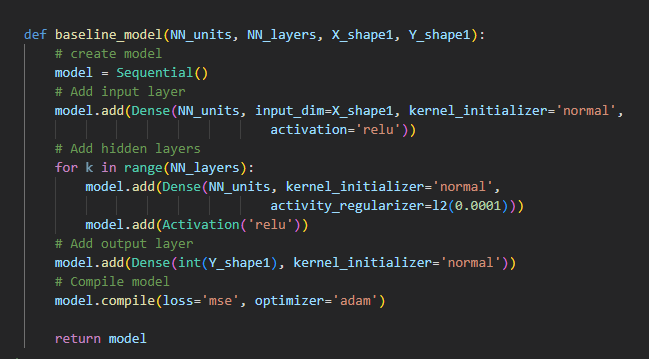
\includegraphics[width=15cm]{Código Red Neuronal función.png}
\end{figure}

\begin{figure}[H]
	\centering
	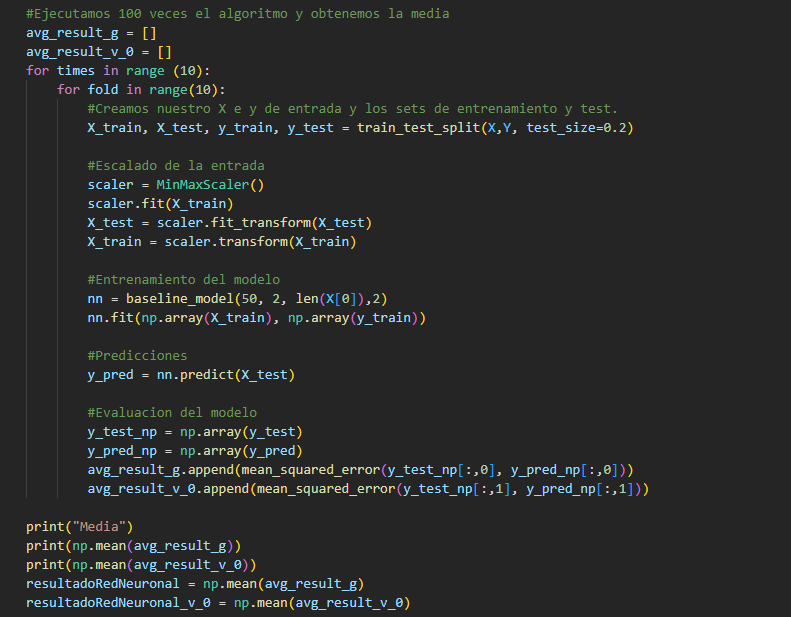
\includegraphics[width=15cm]{Código Red Neuronal.png}
\end{figure}

\begin{figure}[H]
	\centering
	\includegraphics[width=11cm]{Red Neuronal Variable g.png}
\end{figure}

\begin{figure}[H]
	\centering
	\includegraphics[width=12cm]{Red Neuronal Variable v_0.png}
\end{figure}

\subsection{Machine Learning con algoritmo no lineal - red neuronal aplicando autocorrelación}

\begin{figure}[H]
	\centering
	\includegraphics[width=11cm]{Red Neuronal aplicando autocorrelación Variable g.png}
\end{figure}

\begin{figure}[H]
	\centering
	\includegraphics[width=12cm]{Red Neuronal aplicando autocorrelación Variable v_0.png}
\end{figure}

\section{Comparación de los resultados de errores cuadráticos medios}

Después de haber ejecutado un total de $1000$ veces cada algoritmo con distintos datos de entrenamiento y de test se ha calculado la media de los errores cuadráticos de cada uno de ellos, tanto para la variable g como variable $v_0$. Dado que los resultados de g y $v_0$ son proporcionales, sólo se mostraran los resultados de una de ellas, en este caso, la variable g.

Una vez almacenados todos estos resultados se han ido comparando en diversas gráficas antes y después de aplicar autocorrelación, siendo los siguientes los resultados obtenidos.

\begin{figure}[H]
	\centering
	\includegraphics[width=11cm]{Todos los resultados.png}
\end{figure}

Se observa claramente que el resultado obtenido con regresión lineal es el peor resultado, llegando aproximadamente a un error cuadrático medio de treinta. Es el resultado esperado pues es el algoritmo más simple y el que menos complejidad algoritmica tiene.

\begin{figure}[H]
	\centering
	\includegraphics[width=11cm]{Todos los resultados con autocorrelación.png}
\end{figure}

Aunque mejora considerablemente el error cuadrático medio después de aplicar autocorrelación, seguimos sin obtener un resultado capaz de ser comparado con el obtenido en el resto de algoritmos. Por ello, para la siguiente gráfica, será excluido para conseguir una mejor comparativa.

\begin{figure}[H]
	\centering
	\includegraphics[width=11cm]{Todos los resultados sin regresión lineal simple.png}
\end{figure}

En esta gráfica ya si podemos observar errores cuadráticos medios por debajo de uno, lo cual son resultados bastane buenos, sin embargo, observamos que el algorimto de K-NNeighbors es el que obtiene el mejor resultado seguidos por los algoritmos de Ridge.

\begin{figure}[H]
	\centering
	\includegraphics[width=11cm]{Todos los resultados sin regresión lineal simple con autocorrelación.png}
\end{figure}

Después de aplicar autocorrelación, observamos que el algoritmo de machine learning basado en la Red Neuronal no es capaz de generar buenos resultados por lo tanto será excluido en la siguiente comparativa.

\begin{figure}[H]
	\centering
	\includegraphics[width=11cm]{Mejores resultados.png}
\end{figure}

\begin{figure}[H]
	\centering
	\includegraphics[width=11cm]{Mejores resultados con autocorrelación.png}
\end{figure}

Al quedarnos únicamente con los cinco algoritmos con los que se han obtenido los mejores resultados, se puede observar que el algoritmo de K-NNeighbors es el que obtiene mejores resultados siendo su error cuadrático medio de $0.1$ antes de aplicar autocorrelación y muy próximo a $0.055$, mientras que los algoritmos de Ridge únicamente se acercan a $0.1$ después de haber aplicado autocorrelación.

\chapter{Conclusiones}\label{part:conclusiones}

\section{Relevancia del TFG para la neurociencia y la medicina}

Gracias a las simulaciones del modelo cerebral hemos sido capaces de, en primer lugar, obtener un gran conjunto de datos, entre ellos la señal del electroencefalograma, que es una de las señales no-invasivas más conocida en el ámbito clínico. En segundo lugar, analizando estas señales hemos sido capaces de detectar diferentes tipos de gráficas, algunas muy realistas y otras, sin embargo, que serían prácticamente imposible de obtener en la vida real pero que han sido de utilidad para entender entre que rangos de valores debemos de trabajar.

Posteriormente, hemos estudiado si es posible realmente estimar los parámetros del modelo, como el cociente de excitación, E, e inhibición: E/I, que ha dado lugar a las distintas propiedades de la señal del EEG. Mediante herramientas de machine learning (ML), hemos podido encontrar automáticamentelas  regiones de interés del espacio de parámetros del modelo cortical y que se relacionan con cambios en la señal del EEG.

Es imporante remarcar que gracias a este estudio, hemos sido capaces de estudiar que las variaciones del parámetro E/I pueden influir directamente en el diagnóstico de algunas enfermedades como la epilepsia o el autismo. De tal forma que cuando se aumenta el cociente E/I, existe una mayor probabilidad de que se dén enfermedades como la epilepsia en la cual, hay un gran aumento de la actividad neuronal, o de igual forma al disminuir este cociente E/I, existe una mayor probabilidad de que dén enfermedades como el autismo, donde se puede se produce una disminución considerable de actividad neuronal, como se demuestra en el modelo del artículo \cite{modelofautism}.

Gracias a la herramienta desarrollada en este tfg, hemos sido capaces de, usando un modelo del cerebro, poder leer señales del EEG y producir estimaciones de cambios en E/I. De tal forma que a partir de los resultados obtenidos en las simulaciones y tras hacer un estudio de los mejores algoritmos de machine learning, se ha podido obtener con bastante exactitud cual sería su correspondiente cociente E/I.

Finalmente, indicar también que hemos tenido algunas limitaciones durante el desarrollo del proyecto ya que el modelo cerebral usado es un modelo simplificado de una pequeña parte del cerebro y no tiene en cuenta conexiones con otras regiones del cerebro, como puede ser por ejemplo, los impulsos procedentes del tálamo. Además el modelo usa neuronas de tipo de LIF, que son neuronas simplificadas, que facilitan el cálculo del potencial con vistas a su implementación hardware, reduciendo el uso de recursos lógicos y optimizando la velocidad de operación del sistema. Por otro lado, la fórumla utilizada para generar el EEG, es una fórmula simplificada, con la que hemos sido capaces de mantenernos cercanos a los valores esperados pero que, sin embargo, no tiene en cuenta otros factores que pueden influir en su resultado.

\chapter{Trabajo futuro}\label{part:futuro}

Como continuación de este trabajo de fin de grado y como en cualquier otro proyecto de investigación, existen diversas líneas de investigación que quedan abiertas y en las que es posible continuar trabajando. En este caso, en el futuro se pueden trabajar en 2 líneas de mejora:

- Mejorar el modelo superando las limitaciones mencionadas anteriormente, haciendo uso de una mayor cantidad de parámetros (por ejemplo, impulsos provenientes del tálamo), los cuales se pueden modificar en las simulaciones con NEST y así obtener una mayor variedad de resultados. De ésta forma se podría estudiar que influencia tienen sobre el resto de parámetros estudiados.

- Aplicar el modelo a registros reales de señales del EEG tomados en pacientes con patologías clínicas. De esta forma, se podría observar si realmente el modelo es capaz de analizar los datos del EEG para estudiar la probabilidad de que un paciente sufra una determinada enfermedad.

\bibliographystyle{plainnat}
\bibliography{bibliography/research}

\addtocontents{toc}{\vspace{1\baselineskip}}

\addcontentsline{toc}{chapter}{\textsc{bibliografía}}

\ctparttext{\color{black}\begin{center}
\end{center}}

%\addtocontents{toc}{\vspace{1\baselineskip}}

%\clearpage

%\printglossary[title={\textsc{notación}}]
%\glsaddallunused


\end{document}